\documentclass[10pt, oneside]{book}
\usepackage{xeCJK}
\usepackage{amsmath, amsthm, amssymb, bm, graphicx, hyperref, mathrsfs}
\usepackage{geometry}
% \geometry{b5paper,scale=0.85}
\geometry{b5paper,left=1.2cm,right=1.2cm,top=2cm,bottom=1cm}
\usepackage{graphicx} %插入图片的宏包
\usepackage{float} %设置图片浮动位置的宏包
\usepackage{subfigure} %插入多图时用子图显示的宏包
\usepackage{amstext} %公式中包含文字的宏包
\usepackage{booktabs} %插入表格的宏包
\usepackage{multirow} 
\usepackage{indentfirst} %设置缩进的宏包
\setlength{\parindent}{2em}
\usepackage{enumerate} %用于编号的宏包
\usepackage{hyperref} %用于引用的宏包
% \hypersetup{colorlinks, linkcolor=blue} %设置引用的字体颜色
\usepackage{color} %用于设置字体颜色的宏包



% 封面部分
\title{\Huge{\textbf{ROS Notebook}}}
\author{Wu Yutian}
\date{2021.11.13}
\linespread{1.4}
\newtheorem{theorem}{定理}[section]
\newtheorem{definition}[theorem]{定义}
\newtheorem{lemma}[theorem]{引理}
\newtheorem{corollary}[theorem]{推论}
\newtheorem{example}[theorem]{例}
\newtheorem{proposition}[theorem]{命题}
\begin{document}

% 输出封面
\maketitle

% 前言部分
\pagenumbering{roman}
\setcounter{page}{1}

\begin{center}
    \Huge\textbf{前言}
\end{center}~\

主要参考了胡春旭的《ROS机器人开发实践》一书。

~\\
\begin{flushright}     
    \begin{tabular}{c}
        Wu Yutian\\
        2021.11.13
    \end{tabular}
\end{flushright}

\newpage
\pagenumbering{Roman}
\setcounter{page}{1}
\tableofcontents
\newpage
\setcounter{page}{1}
\pagenumbering{arabic}

% -------------------------chapter 1-------------------------
\chapter{ROS的基本架构——ROS1}

\section{整体架构}

\begin{figure}[H]
    \centering
    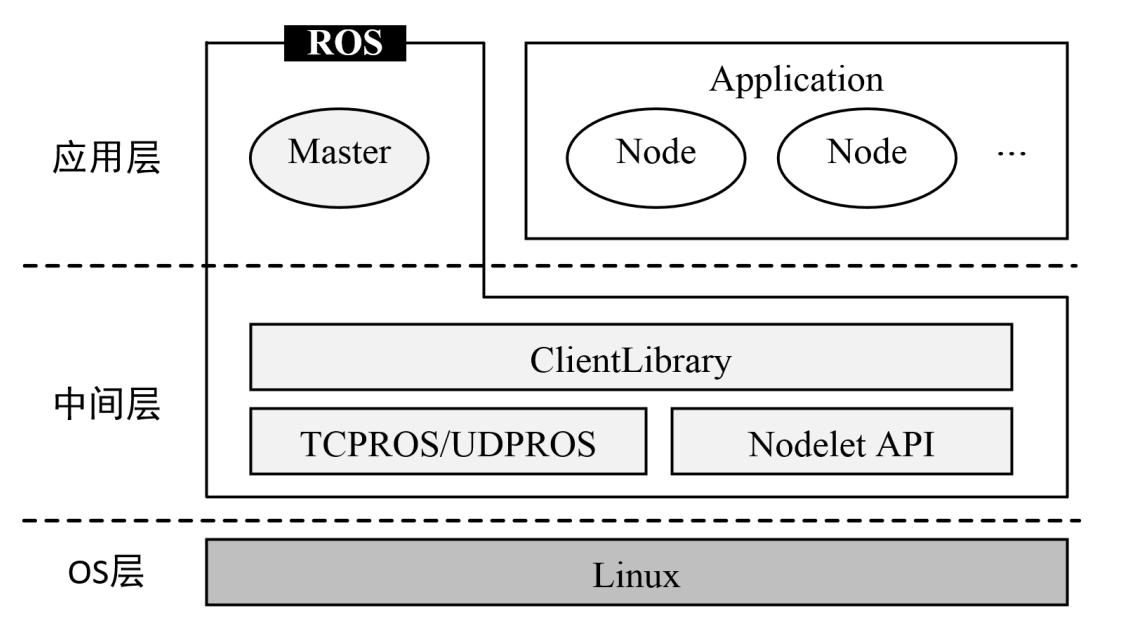
\includegraphics[width=0.6\linewidth]{image/ROS1架构.jpg}
\end{figure}

OS层:是ROS依托的底层操作系统,一般是Ubuntu。

中间层:最重要的就是基于TCP/UDP网络,进行封装形成的TCPROS/UDPROS通信系统,这其中包括了Topic的发布、订阅的通信方式,Service的客户端、服务器的通信方式等。另外ROS还提供了一种进程内通信的方式——Nodelet,可以为多进程通信提供一种更优化的数据传输方式,适合对实时性要求较高的应用。

在通信机制的基础上,ROS还在中间层提供了大量的机器人开发相关的实用功能,如:数据类型定义、坐标变换、运动控制等。

应用层:ROS需要运行一个管理者——Matser,负责整个系统的正常运行。其他的一些相关的ROS功能包都是以节点(Node)的方式运行,一般来说,简单的开发工作只需要关注节点的标准输入输出接口,而不需要关注模块的内部实现。

\section{计算图的视角}

\begin{figure}[H]
    \centering
    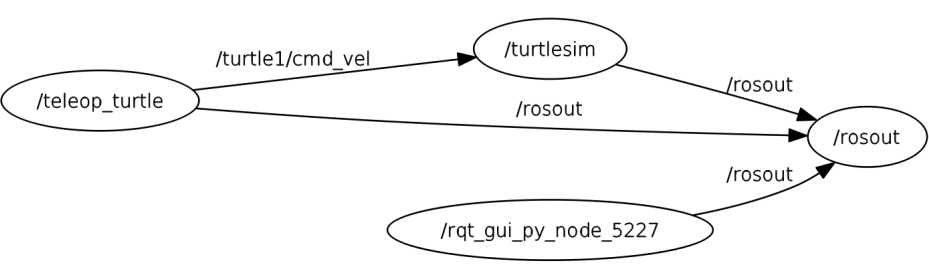
\includegraphics[width=0.7\linewidth]{image/计算图.png}
\end{figure}

从计算图的视角来看ROS的功能模块,它们都是以节点为单位独立运行的,甚至可以分布于不同的主机中。

\subsection{节点 Node}

节点就是一些执行运算任务的进程,它们之间可以相互通信。

\subsection{话题 Topic}

消息以一种发布/订阅(publish/subscribe)的方式传递,发布者和订阅者并不了解彼此的存在,系统中可能有多个节点发布或者订阅同一个话题的消息。

\subsection{服务 Service}

对于双向的同步传输模式,采用基于客户端/服务器(Client/Server)的模型,包含请求和应答,类似于Web服务器,ROS中只允许有一个节点提供指定命名的服务。

\subsection{节点管理器 Master}

节点管理器帮助ROS节点之间相互查找、建立连接,同时还为系统提供参数服务器,管理全局参数。

\section{文件系统}

\subsection{功能包}

功能包相关的常用ROS命令:

\begin{table}[H]
    \centering
    \begin{tabular}{c|c}
    \hline
    命令                  & 作用            \\ \hline
    catkin\_create\_pkg & 创建功能包         \\
    rospack             & 获取功能包的信息      \\
    catkin\_make        & 编译功能包的信息      \\
    rosdep              & 自动安装功能包依赖的其他包 \\
    roscd               & 功能包目录跳转       \\
    roscp               & 拷贝功能包中的文件     \\
    rosed               & 编辑功能包中的文件     \\
    rosrun              & 运行功能包中的可执行文件  \\
    roslaunch           & 运行启动文件        \\ \hline
    \end{tabular}
\end{table}

\section{通信机制}

\subsection{话题通信机制——Topic}

\begin{figure}[H]
    \centering
    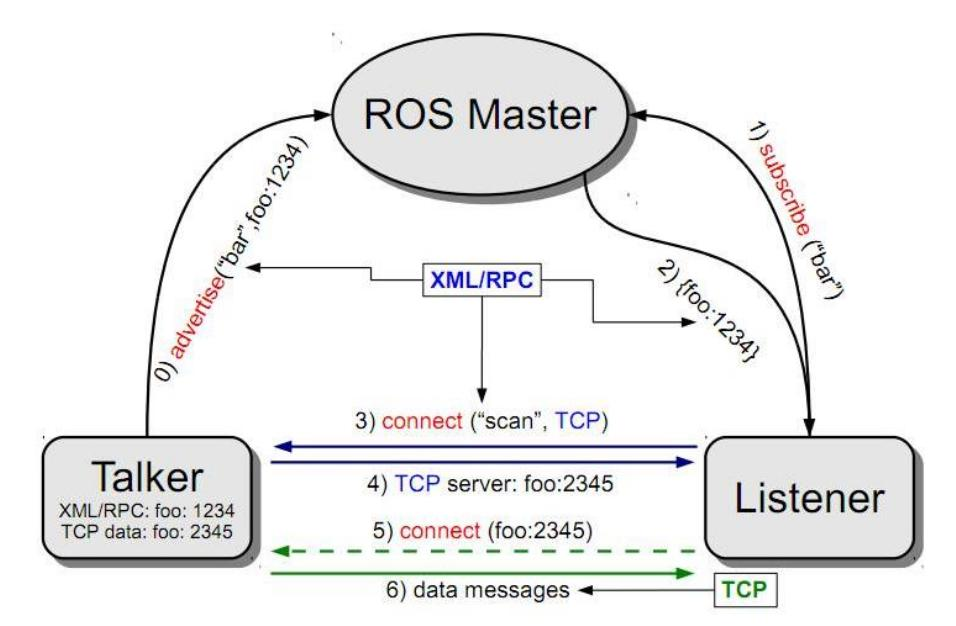
\includegraphics[width=0.7\linewidth]{image/话题通信机制.jpg}
\end{figure}

假设Talker首先启动,建立通信的详细过程:

\begin{itemize}
    \item 1、发布者(Talker)启动,通过RPC向 ROS Master 注册发布者的信息,包括:发布者节点信息,话题名,话题缓存大小等;Master 会将这些信息加入注册列表中;
    \item 2、订阅者(Listener)启动,通过 RPC 向 ROC Master 注册订阅者信息,包括:订阅者节点信息,话题名等;Master 会将这些信息加入注册列表;
    \item 3、Master 进行节点匹配:Master 会根据订阅者提供的信息,在注册列表中查找匹配的发布者;如果没有发布者(Talker),则等待发布者(Talker)的加入;如果找到匹配的发布者(Talker),则会主动把发布者(Talker)(有可能是很多个 Talker)的地址通过 RPC 传送给订阅者(Listener)节点;
    \item 4、Listener 接收到 Master 的发出的 Talker 的地址信息,尝试通过 RPC 向 Talker 发出连接请求(信息包括:话题名,消息类型以及通讯协议(TCP/UDP));
    \item 5、Talker 收到 Listener 发出的连接请求后,通过 RPC 向 Listener 确认连接请求(包含的信息为自身 TCP 地址信息);
    \item 6、Listener 接收到 Talker 的确认消息后,使用 TCP 尝试与 Talker 建立网络连接;
    \item 7、成功连接之后,Talker 开始向 Listener 发布话题消息数据;
\end{itemize}

需要注意的是:有可能多个 Talker 连接一个 Listener,也有可能是一个 Talker 连接上多个 Listener(多对多)。

\subsection{服务通信机制——Service}

\begin{figure}[H]
    \centering
    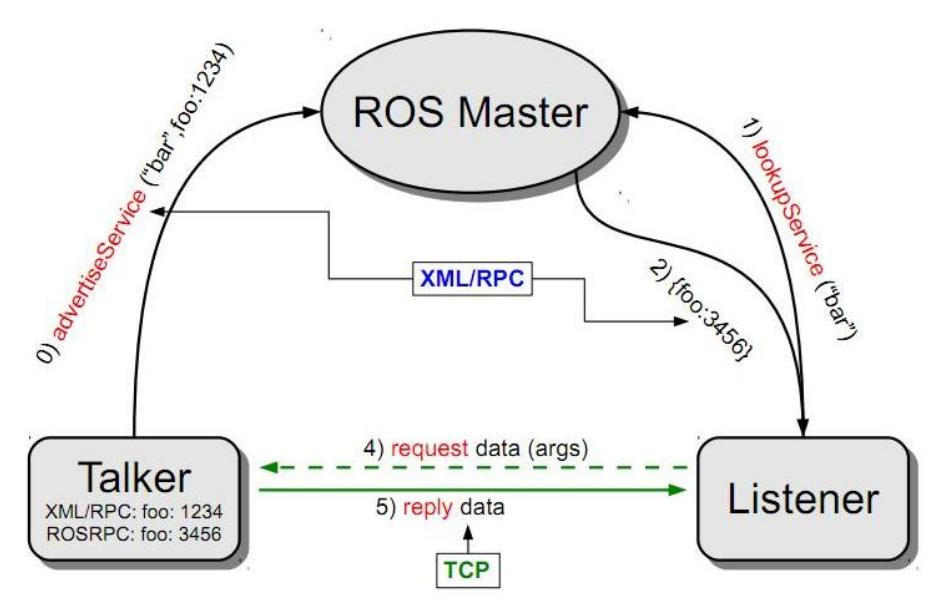
\includegraphics[width=0.7\linewidth]{image/服务通信机制.jpg}
\end{figure}

与话题的通信相比,其减少了Listener与Talker之间的RPC通信,建立通信的详细过程:

\begin{itemize}
    \item 1、发布者(Talker)启动,通过RPC向 ROS Master 注册发布者的信息,包括:发布者节点信息,话题名,话题缓存大小等;Master 会将这些信息加入注册列表中;
    \item 2、订阅者(Listener)启动,通过 RPC 向 ROC Master 注册订阅者信息,包括:订阅者节点信息,话题名等;Master 会将这些信息加入注册列表;
    \item 3、Master 进行节点匹配:Master 会根据订阅者提供的信息,在注册列表中查找匹配的发布者;如果没有发布者(Talker),则等待发布者(Talker)的加入;如果找到匹配的发布者(Talker),则会主动把发布者(Talker)(有可能是很多个 Talker)的地址通过 RPC 传送给订阅者(Listener)节点;
    \item 4、Listener 接收到 Talker 的确认消息后,使用 TCP 尝试与 Talker 建立网络连接;
    \item 5、成功连接之后,Talker 开始向 Listener 发布话题消息数据;
\end{itemize}

需要注意的是:有可能是一个 Talker 连接上多个 Listener(一对多)。

\subsection{参数管理机制——Parameter}

\begin{figure}[H]
    \centering
    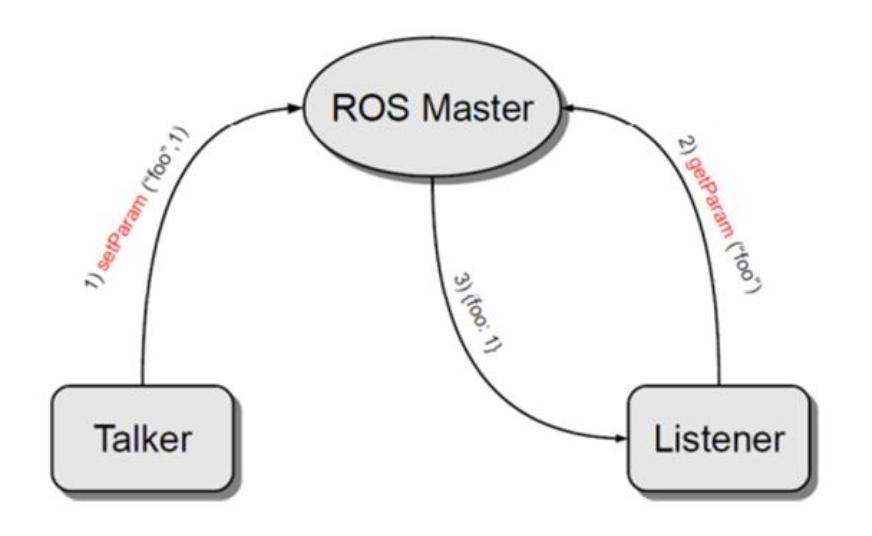
\includegraphics[width=0.7\linewidth]{image/参数管理机制.jpg}
\end{figure}

参数共享机制类似于程序中的全局变量,Talker 去更新全局变量(共享的参数),Listener 去获取更新后的全局变量(共享的参数);这个通信过程不涉及 TCP/UDP 的通信;     

\begin{itemize}
    \item 1、Talker 更新全局变量;Talker 通过 RPC 更新 ROS Master 中的共享参数(包含参数名和参数值);
    \item 2、Listener 通过 RPC 向 ROS Master 发送参数查询请求(包含要查询的参数名);
    \item 3、ROS Master 通过 RPC 回复 Listener 的请求(包括参数值);
\end{itemize}

需要注意的是:如果 Listener 向实时知道共享参数的变化,需要自己不停的去询问 ROS Master;


% -------------------------chapter 2-------------------------
\chapter{ROS基础}

\section{turtlesim功能包}

接触的第一个ROS功能包:turtlesim,其核心是tuetlesim\_node节点。

其中包含的话题和服务如下:

\begin{table}[H]
    \centering
    \begin{tabular}{ccll}
    \hline
                                             & 名称                                               & \multicolumn{1}{c}{类型}                                                                      & \multicolumn{1}{c}{描述}                                                \\ \hline
    \multicolumn{1}{c|}{话题订阅}                & \multicolumn{1}{c|}{turtleX/cmd\_vel}            & \multicolumn{1}{l|}{\begin{tabular}[c]{@{}l@{}}geometry\_msgs/\\ Twist\end{tabular}}        & \begin{tabular}[c]{@{}l@{}}控制乌龟角速度与线速度的\\ 输入指令\end{tabular}           \\ \hline
    \multicolumn{1}{c|}{话题发布}                & \multicolumn{1}{c|}{turtleX/pose}                & \multicolumn{1}{l|}{turtlesim/Pose}                                                         & \begin{tabular}[c]{@{}l@{}}乌龟的姿态信息:包括x与y\\ 坐标、角度、线速度和角速度\end{tabular} \\ \hline
    \multicolumn{1}{c|}{\multirow{7}{*}{服务}} & \multicolumn{1}{c|}{clear}                       & \multicolumn{1}{l|}{std\_srvs/Empty}                                                        & 清楚仿真器中的背景颜色                                                           \\ \cline{2-4} 
    \multicolumn{1}{c|}{}                    & \multicolumn{1}{c|}{reset}                       & \multicolumn{1}{l|}{std\_srvs/Empty}                                                        & 复位仿真器到初始状态                                                            \\ \cline{2-4} 
    \multicolumn{1}{c|}{}                    & \multicolumn{1}{c|}{kill}                        & \multicolumn{1}{l|}{turtlesim/Kill}                                                         & 删除一只乌龟                                                                \\ \cline{2-4} 
    \multicolumn{1}{c|}{}                    & \multicolumn{1}{c|}{spawn}                       & \multicolumn{1}{l|}{turtlesim/Spawn}                                                        & 新生一只乌龟                                                                \\ \cline{2-4} 
    \multicolumn{1}{c|}{}                    & \multicolumn{1}{c|}{turtleX/set\_pen}            & \multicolumn{1}{l|}{turtlesim/Setpen}                                                       & 设置画笔的颜色和线宽                                                            \\ \cline{2-4} 
    \multicolumn{1}{c|}{}                    & \multicolumn{1}{c|}{turtleX/teleport\_absolute}  & \multicolumn{1}{l|}{\begin{tabular}[c]{@{}l@{}}turtlesim/\\ TeleportAbsolute\end{tabular}}  & 移动乌龟到指定的姿态                                                            \\ \cline{2-4} 
    \multicolumn{1}{c|}{}                    & \multicolumn{1}{c|}{turtleX/teleport\_realative} & \multicolumn{1}{l|}{\begin{tabular}[c]{@{}l@{}}turtlesim/\\ TeleportRealative\end{tabular}} & 移动乌龟到指定的角度和距离                                                         \\ \hline
    \end{tabular}
\end{table}

\section{创建工作空间和功能包}

\subsection{创建工作空间}


工作空间初始化:
\begin{verbatim}
    mkdir ~/catkin_ws/src
    cd ~/catkin_ws/src
    catkin_init_workspace
\end{verbatim}

初始化后,可以编译整个工作空间:
\begin{verbatim}
    cd ~/catkin_ws/
    catkin_make
\end{verbatim}

编译后,在工作空间的根目录下会产生build和devel两个文件夹,在devel文件夹中有setup.bash形式的环境变量设置脚本,则可以使用source命令运行这些脚本配置环境变量,如:
\begin{verbatim}
    source devel/setup.bash
\end{verbatim}

但是source命令设置的环境变量只在当前终端中有效,所以为了方便,可以讲终端的配置文件(~/.bashrc)中加入上面的环境变量的配置语句(要注意写全绝对路径)。

\subsection{创建功能包}

创建功能包的命令如下:

\begin{verbatim}
    cd ~/catkin_ws/src
    catkin_create_pkg <package_name> [depend1] [depend2] [depend3]
\end{verbatim}

创建完成后,工作空间的src目录中会生成一个<package\_name>的功能包,并且已经包含了package.xml和CMakelist.txt文件。其中package.xml文件提供描述功能包属性的信息,CMakelist.txt文件记录功能包的编译规则。

进而可以回到工作空间的根目录下进行编译,并设置环境变量。

\section{工作空间的覆盖}

所有工作空间的路径会依次在ROS\_PACKAGE\_PATH环境变量中记录,当设置多个工作空间的环境变量后,新设置的路径在ROS\_PACKAGE\_PATH中会自动放在最前端。在运行时,ROS会优先查找最前端的工作空间中是否存在指定的功能包,如果不存在,就顺序向后查找其他工作空间,知道最后一个工作空间为止。

\section{Topic中的Publisher和Subscriber}

\subsection{Publisher的创建}

\begin{verbatim}
    #include <sstream>
    #include "ros/ros.h"
    #include "std_msgs/String.h"
    int main(int argc, char **argv){
        // ROS节点初始化
        ros::init(argc, argv, "talker");
        // 创建节点句柄
        ros::NodeHandle n;
        // 创建一个Publisher,发布名为chatter的topic,消息类型为std_msgs::String
        ros::Publisher chatter_pub = n.advertise<std_msgs::String>("chatter", 1000);
        // 设置循环的频率
        ros::Rate loop_rate(10);
        int count = 0;
        // 一旦发生异常,ros::ok()就会返回false,跳出循环
        while (ros::ok()){
            // 初始化std_msgs::String类型的消息
            std_msgs::String msg;
            std::stringstream ss;
            ss << "hello world " << count;
            msg.data = ss.str();
            // 发布消息
            ROS_INFO("%s", msg.data.c_str());
            chatter_pub.publish(msg);
            // 循环等待回调函数
            // ros::spinOnce()函数用来处理节点订阅话题的所有回调函数
            // 虽然目前的发布节点并没有任何订阅信息,ros::spinOnce()不是必须的
            // 但是为了保证功能无误,建议所有节点都默认加入该函数
            ros::spinOnce();
            // 按照循环频率延时
            loop_rate.sleep();
            ++count;
        }
        return 0;
    }
\end{verbatim}

\subsection{Subscriber的创建}

\begin{verbatim}
    #include "ros/ros.h"
    #include "std_msgs/String.h"
    // 接收到订阅的消息后,会进入消息回调函数
    // 当有消息到达时,会自动以消息指针作为参数
    void chatterCallback(const std_msgs::String::ConstPtr& msg){
        // 将接收到的消息打印出来
        ROS_INFO("I heard: [%s]", msg->data.c_str());
    }
    int main(int argc, char **argv){
        // 初始化ROS节点
        ros::init(argc, argv, "listener");
        // 创建节点句柄
        ros::NodeHandle n;
        // 创建一个Subscriber,订阅名为chatter的topic,注册回调函数chatterCallback
        ros::Subscriber sub = n.subscribe("chatter", 1000, chatterCallback);
        // 循环等待回调函数
        ros::spin();
        return 0;
    }
\end{verbatim}

\subsection{自定义话题消息}

\subsubsection{编写msg文件}

使用msg文件定义自己的消息类型,一般放置在功能包根目录下的msg文件夹中。msg文件中既可以定义消息类型的变量,也可以定义常量:

\begin{verbatim}
    string name
    uint8  sex
    uint8  age
    
    uint8 unknown = 0
    uint8 male    = 1
    uint8 female  = 2
\end{verbatim}

对于稍复杂一些的ROS自定义消息,还会包含一个标准格式的头信息std\_msgs/Header:
\begin{verbatim}
    unint32 seq
    time stamp
    string frame_id  
\end{verbatim}

其中:seq是消息的顺序标识,不需要手动设置,Publisher在发布消息时会自动累加;stamp是消息中与数据相关联的时间戳,可以用于时间同步;frame\_id是消息中与数据相关联的参考坐标系id。

\subsubsection{编译msg文件}

(1)在package.xml中添加功能包依赖

\begin{verbatim}
    <build_depend>message_generation</build_depend>
    <run_depend>message_runtime</run_depend>
\end{verbatim}

(2)在CMakeLists.txt文件中添加编译选项

在find\_package中添加消息生成依赖的功能包message\_generation:
\begin{verbatim}
    find_package(catkin REQUIRED COMPONENTS
        geometry_msgs
        roscpp
        rospy
        std_msgs
        message_generation
    )
\end{verbatim}

设置catkin依赖:
\begin{verbatim}
    catkin_package(
        # INCLUDE_DIRS include
        # LIBRARIES learning_communication
        CATKIN_DEPENDS geometry_msgs roscpp rospy std_msgs message_runtime
        # DEPENDS system_lib
    )
\end{verbatim}

设置需要编译的msg文件:
\begin{verbatim}
    add_message_files(FILES Person.msg) 
    generate_messages(DEPENDENCIES std_msgs)
\end{verbatim}

然后对功能包进行编译,自定义的消息类型就生效了。

\subsection{CMakeLists的编写}

几个常用的编译选项:

(1)include\_directories

用于设置头文件的相对路径。功能包的一些头文件会放在功能包根目录下的include文件夹中,所以需要添加该文件夹。

(2)add\_executable

用于设置需要编译的代码和生成的可执行文件。第一个参数为期望生成的可执行文件的名称,后面的参数为参与的源码文件(cpp),如果需要多个代码文件,可以在后面依次列出,中间用空格分隔。

(3)target\_link\_libraries

用于设置链接库。第一个参数为期望生成的可执行文件的名称,后面依次列出需要链接的库,如果没有使用其他库,添加默认链接库(\$\{catkin\_LIBRARIES\})即可。

(4)add\_dependencies

用于设置依赖。在很多应用中,我们需要定义语言无关的消息类型,消息类型会在编译过程中产生相应语言的代码,如果编译的可执行文件依赖这些动态生成的代码,则需要使用add\_dependencies添加\$\{PROJECT\_NAME\}\_generate\_messages\_cpp配置,即该功能包动态产生的消息代码。

对于我们的这个例子,CMakeLists.txt文件如下:

\begin{verbatim}
    include_directories(include ${catkin_INCLUDE_DIRS})

    add_executable(talker src/talker.cpp)
    target_link_libraries(talker ${catkin_LIBRARIES})
    add_dependencies(talker ${PROJECT_NAME}_generate_messages_cpp)
      
    add_executable(listener src/listener.cpp)
    target_link_libraries(listener ${catkin_LIBRARIES})
    add_dependencies(talker ${PROJECT_NAME}_generate_messages_cpp)
\end{verbatim}


\section{Service中的Client和Server}

\subsection{创建Client}

\begin{verbatim}
    #include <cstdlib>
    #include "ros/ros.h"
    #include "learning_communication/AddTwoInts.h"
    
    int main(int argc, char **argv){
        ros::init(argc, argv, "add_two_ints_client");
        // 从终端命令行获取两个加数,argv[0]是路径,argv[1]和[2]是两个输入参数
        if (argc != 3){
            ROS_INFO("usage: add_two_ints_client X Y");
            return 1;
        }
        ros::NodeHandle n;    
        // 创建一个client,请求add_two_int service
        // service消息类型是learning_communication::AddTwoInts
        ros::ServiceClient client = n.serviceClient\
            <learning_communication::AddTwoInts>("add_two_ints");
        // 创建learning_communication::AddTwoInts类型的service消息
        // 该变量包含两个成员:request和response
        learning_communication::AddTwoInts srv;
        // atoll()函数将字符串转化为整数
        srv.request.a = atoll(argv[1]);
        srv.request.b = atoll(argv[2]);
        // 发布service请求,等待加法运算的应答结果
        // 调用过程会发生阻塞,调用成功后返回true
        if (client.call(srv)){
            ROS_INFO("Sum: %ld", (long int)srv.response.sum);
        }
        else{
            ROS_ERROR("Failed to call service add_two_ints");
            return 1;
        }
        return 0;
    }
\end{verbatim}

\subsection{创建server}

\begin{verbatim}
    #include "ros/ros.h"
    #include "learning_communication/AddTwoInts.h"
    // service回调函数,输入参数req,输出参数res
    bool add(learning_communication::AddTwoInts::Request  &req,
             learning_communication::AddTwoInts::Response &res){
        // 将输入参数中的请求数据相加,结果放到应答变量中
        res.sum = req.a + req.b;
        ROS_INFO("request: x=%ld, y=%ld", (long int)req.a, (long int)req.b);
        ROS_INFO("sending back response: [%ld]", (long int)res.sum);
        return true;
    }
    int main(int argc, char **argv){
        ros::init(argc, argv, "add_two_ints_server");
        ros::NodeHandle n;
        // 创建一个名为add_two_ints的server,注册回调函数add()
        ros::ServiceServer service = n.advertiseService("add_two_ints", add);
        // 循环等待回调函数
        ROS_INFO("Ready to add two ints.");
        ros::spin();
        return 0;
    }    
\end{verbatim}

\subsection{自定义服务数据}

\subsubsection{编写srv文件}

使用 srv 文件定义自己的消息类型,一般放置在功能包根目录下的 srv 文件夹中。该文件包含request和response两个数据域,两个数据域之间用"---"(三个减号)分隔,如:

\begin{verbatim}
    int64 a
    int64 b
    ---
    int64 sum
\end{verbatim}

\subsubsection{编译srv文件}

(1)在 package.xml 中添加功能包依赖(与自定义话题消息相同)

\begin{verbatim}
    <build_depend>message_generation</build_depend>
    <run_depend>message_runtime</run_depend>
\end{verbatim}

(2)在CMakeLists.txt文件中添加编译选项

与自定义话题消息相同也是添加message\_generation包,

\begin{verbatim}
    find_package(catkin REQUIRED COMPONENTS
        geometry_msgs
        roscpp
        rospy
        std_msgs
        message_generation
    )
    add_service_files(FILES AddTwoInts.srv)
\end{verbatim}

\subsection{CMakeLists的编写}

与Topic类似:

\begin{verbatim}
    include_directories(include ${catkin_INCLUDE_DIRS})
            
    add_executable(server src/server.cpp)
    target_link_libraries(server ${catkin_LIBRARIES})
    add_dependencies(server ${PROJECT_NAME}_gencpp)

    add_executable(client src/client.cpp)
    target_link_libraries(client ${catkin_LIBRARIES})
    add_dependencies(client ${PROJECT_NAME}_gencpp)
\end{verbatim}

\section{ROS中的命名空间}

\subsection{有效的命名}

\begin{itemize}
    \item 1、首字符必须是([a-z|A-Z])、波浪线(\textasciitilde)或者左斜杠(/)
    \item 2、后续字母可以是字母或数字([0-9|a-z|A-Z])、下划线(\_)或者左斜杠
\end{itemize}

\subsection{命名解析}

\subsubsection{全局名称:/global/name}

全局名称的首字符是左斜杠,它之所以称为全局,是因为它的解析度最高,可以在全局范围内直接访问。

但是在系统中,全局名称越少越好,因为过多的全局名称会影响功能包的可移植性。

\subsubsection{相对名称:relative/name}

相对名称由ROS提供默认的命名空间,不需要带有开头的左斜杠,ROS会对一个相对名称进行解析,进而得到一个全局名称来使用,就类似与我们平时使用的相对路径。相对名称的使用会提高可移植性。

例如:在默认命名空间/relative内使用相对名称name,则系统会将其解析为全局名称:/relative/name。

ROS提供的三种指定默认命名空间的方式:

\begin{itemize}
    \item[-] 1、通过命令参数设置

    调用ros::init()的程序会接受一个名为\_\_ns的命令行参数,用来设置默认命名空间:

\begin{verbatim}
__ns:=deflaut-namespace
\end{verbatim}

    \item[-] 2、在launch文件中设置
    
    在launch文件中可以通过参数ns来设置默认命名空间:

\begin{verbatim}
<node pkg="turtlesim" type="turtlesim_node" name="turtlesim\_node" ns="sim1"/>
\end{verbatim}

    \item[-] 3、使用环境变量设置
    
    在执行ROS程序的终端中设置默认命名空间的环境变量:

\begin{verbatim}
export ROS_NAMESPACE = default-namespace
\end{verbatim}


\end{itemize}

\subsubsection{私有名称:~private/name}

私有名称是一个节点内部私有的资源名称,只会在节点内部使用。私有名称以波浪线“\textasciitilde”开始。类似相对名称,也需要ROS为其解析,成为一个有意义的全局名称,不同的是,私有名称并不使用当前的默认命名空间,而是使用节点的全局名称作为命名空间。

例如有一个节点的全局名称是/sim1/pubvel,其中的一个私有名称为\textasciitilde/max\_vel,则其会被解析成全局名称:/sim1/pubvel/max\_vel。

\subsubsection{ROS命名解析总结}

\begin{table}[H]
    \begin{tabular}{c|c|c|c}
    \hline
    节点        & 全局名称                            & 相对名称(默认)                         & 私有名称                                         \\ \hline
    /node1    & /bar -\textgreater /bar         & Bar -\textgreater /bar           & $\sim$bar -\textgreater /node1/bar           \\ \hline
    /wg/node2 & /bar -\textgreater /bar         & Bar -\textgreater /wg/bar        & $\sim$bar -\textgreater wg/node2/bar         \\ \hline
    /wg/node3 & /foo/bar -\textgreater /foo/bar & foo/bar -\textgreater wg/foo/bar & $\sim$foo/bar -\textgreater wg/node3/foo/bar \\ \hline
    \end{tabular}
\end{table}

\subsection{命名重映射}

所有的ROS节点内的资源名称都可以在节点启动的时候进行重映射,这一特性支持我们同事打开多个相同的节点,而不会发生命名冲突。

命名重映射语法:

\begin{verbatim}
    old\_name:=new\_name
\end{verbatim}

例如,要将chatter重映射为/wg/chatter,在节点启动时候可以输入如下命令:

\begin{verbatim}
    $ rosrun rospy_tutorials talker chatter:=/wg/chatter 
\end{verbatim}

需要注意:ROS的命名解析是在命名重映射之前发生的。所以当我们使用“foo:=bar”时,会将节点内所有foo命名映射为bar,而如果我们重映射“/foo:=bar”时,ROS只会讲全局解析为/foo的名称重映射为bar。

命名重映射和命名解析之间的关系:

\begin{table}[H]
    \centering
    \begin{tabular}{c|c|c|c}
    \hline
    节点命名空间 & 重映射参数            & 匹配名称         & 解析名称       \\ \hline
    /      & foo:=bar         & foo,/foo     & /bar       \\ \hline
    /baz   & foo:=bar         & foo,/baz/foo & /baz/bar   \\ \hline
    /      & /foo:=bar        & foo,/foo     & /bar       \\ \hline
    /baz   & /foo:=bar        & /foo         & /baz/bar   \\ \hline
    /baz   & /foo:=/a/b/c/bar & /foo         & /a/b/c/bar \\ \hline
    \end{tabular}
\end{table}

\section{多机通信}

\subsubsection{设置IP地址}

\begin{itemize}
    \item 1、确保所有计算机处于同一网络中,使用ifconfig命令查看本机的局域网ip地址。
    \item 2、分别在每台计算机的/etc/hosts文件中添加其他计算机的ip地址和对应的计算机名称。
    \item 3、测试是否能够ping通其他计算机。
\end{itemize}

\subsubsection{设置ROS\_MASTER\_URI}

因为系统中只能存在一个Master,所以从机需要知道Master的位置,可以在从机中使用如下命令,将Master的地址写入环境变量中:

\begin{verbatim}
    $ echo "export ROS_MASTER_URI = http://<主机名>::11311" >> ~/.bashrc
\end{verbatim}


% -------------------------chapter 3-------------------------
\chapter{ROS中的常用组件}

\section{launch文件}

launch文件是ROS中同时启动多个节点的途径,它还可以自动启动ROS Master节点管理器,并且实现每个节点的各种配置。

launch文件采用XML的形式进行描述,XML文件必须包含一个根元素,launch文件的根元素采用<launch>标签定义,文件中的其他内容都必须包含在这个标签中。

\subsection{启动节点}

采用<node>标签启动ROS节点,语法如下:

\begin{verbatim}
    <node pkg = "package-name" type = "executable-name" name = "node-name"/>
\end{verbatim}

\begin{itemize}
    \item pkg定义节点所在的功能包名称
    \item type定义节点的可执行文件名称
    \item name定义节点运行时的名称,讲覆盖节点中init()赋予节点的名称
\end{itemize}

另外还有如下可选的属性参数:

\begin{itemize}
    \item output = "screen":讲节点的标准输出打印到终端(默认输出为日志文档)
    \item respawn = "true":复位属性,该节点停止时,会自动重启,默认为flase
    \item required = "true":必要节点,当该节点终止时,launch文件中的其他节点也被终止
    \item ns = "namespace":命名空间,为节点内的相对名称添加命名空间前缀
    \item args = "arguments":节点需要输入的参数
\end{itemize}

\subsection{系统参数设置}

使用<param>标签来设置ROS系统运行中的参数(即parameter),存储在参数服务器中。launch文件执行后,parameter就加载到ROS的参数服务器上。

每个活跃的节点都可以通过ros::param::get()接口来获取parameter的值,用户也可以在终端中通过rosparam命令获得parameter的值。

<param>标签的语法如下:

\begin{verbatim}
    <param name = "output_frame" value = "odom"/>
\end{verbatim}

另外,ROS也提供了一种从文件中批量加载参数的方法,使用标签<rosparam>,其语法如下:

\begin{verbatim}
    <rosparam file = "$(find 2dnav_pr2)/config/costmap_common_params.yamls" command
 = "load" ns = "local_costmap"/>
\end{verbatim}

<rosparam>标签可以帮我们将一个YAML格式的文件中的全部参数加载到ROS中,需要将command属性设置为"load"。

\subsection{设置内部变量}

使用<arg>标签可以设置launch文件内部的局部变量(argument),仅限于launch文件内部使用,语法如下:

\begin{verbatim}
    <arg name = "arg-name" default = "arg-value"/>
\end{verbatim}

在launch文件中使用argument时,可以使用如下语法进行调用:

\begin{verbatim}
    <node pkg = "package" type = "type" name = "name" args = "$(arg arg-name)"/>
\end{verbatim}

\subsection{重映射机制}

使用<remap>标签可以实现重映射的功能,可以给功能包的接口名称重映射一下,取一个别名,可以用来实现不同功能包之间的接口匹配,语法如下:

\begin{verbatim}
    remap from = "turtlebot/cmd_vel" to = "/cmd_vel"/>
\end{verbatim}

\subsection{嵌套复用}

使用<include>标签可以实现在一个launch文件中包含其他的launch文件。即可直接复用其他已有的launch文件中的内容,语法如下:

\begin{verbatim}
    <include file = "$(dirname)/other.launch"/>
\end{verbatim}

\section{TF坐标变换}

TF是一个让用户随时间跟踪多个坐标系的功能包,它使用树形数据结构,根据时间缓冲并维护多个坐标系之间的坐标变换关系。

\subsection{TF辅助工具}

\subsubsection{1.tf\_monitor}

功能是打印TF树中所有坐标系的发布状态,使用方法如下:

\begin{verbatim}
    $ tf_monitor
    $ tf_monitor <source_frame> <target_frame>
\end{verbatim}

\subsubsection{2.tf\_echo}

功能是查看指定坐标系之间的变换关系,使用方法如下:

\begin{verbatim}
    $ tf_echo <source_frame> <target_frame>
\end{verbatim}

\subsubsection{3.static\_transform\_publisher?}

功能是发布两个坐标系之间的静态坐标变换,这两个坐标系不发生相对的位置变化,使用方法如下:

\begin{verbatim}
    $ static_transform_publisher x y z yaw pitch roll frame_id child_frame_id 
period_in_ms
    $ static_transform_publisher x y z qx qy qz qw frame_id child_frame_id 
period_in_ms
\end{verbatim}

以上两种命令格式,需要设置坐标的偏移参数和旋转参数:偏移参数使用相对于xyz轴的坐标位移;旋转参数分别采用了欧拉角和四元数的表达方式,并设置发送频率以ms为单位。

另外,该命令还可以在launch文件中使用,语法如下:

\begin{verbatim}
    <launch>
    <node pkg = "tf" type = "static_transform_publisher" name = "link1_broadcaster" 
args = "1 0 0 0 0 0 1 link1_parent link1 100"/>
    <\launch>
\end{verbatim}

\subsubsection{4.view\_frame}

这是一个可视化的调试工具,可以生成PDF文件,显示整棵TF树的信息,使用方法如下:

\begin{verbatim}
    $ rosrun tf view_frames
\end{verbatim}

\subsection{TF中的Boardcaster和Listener}

以基于TF的乌龟自动跟踪例程为例。

\subsubsection{创建Broadcaster}

创建一个发布乌龟坐标系与世界坐标系之间的TF变换的节点。

\begin{verbatim}
    #include <ros/ros.h>
    #include <tf/transform_broadcaster.h>
    #include <turtlesim/Pose.h>
    std::string turtle_name;
    //回调函数
    void poseCallback(const turtlesim::PoseConstPtr& msg){
        // tf广播器
        static tf::TransformBroadcaster br;
        // 根据乌龟当前的位姿,设置相对于世界坐标系的坐标变换
        // setOrigin设置平移变换 setRotation设置旋转变换
        tf::Transform transform;
        transform.setOrigin( tf::Vector3(msg->x, msg->y, 0.0) );
        tf::Quaternion q;
        q.setRPY(0, 0, msg->theta);
        transform.setRotation(q);
        // 发布坐标变换 TF消息的数据类型为tf::StampedTransform
        // 包含坐标变换、时间戳,并指定坐标变换的源坐标系(parent)和目标坐标系(child)
        br.sendTransform(tf::StampedTransform(transform, ros::Time::now(), "world", 
    turtle_name));
    }
    int main(int argc, char** argv){
        // 初始化节点
        ros::init(argc, argv, "my_tf_broadcaster");
        if (argc != 2){
            ROS_ERROR("need turtle name as argument"); 
            return -1;
        };
        turtle_name = argv[1];
        ros::NodeHandle node;
        // 订阅乌龟的pose信息 订阅到之后,就会进入回调函数进行TF广播
        ros::Subscriber sub = node.subscribe(turtle_name+"/pose", 10, &poseCallback);
        ros::spin();
        return 0;
    };
\end{verbatim}

\subsubsection{创建Listener}

监听TF消息,并且从中获取turtle2相对于turtle1坐标系的变换,从而控制turtle2移动。

\begin{verbatim}
    #include <ros/ros.h>
    #include <tf/transform_listener.h>
    #include <geometry_msgs/Twist.h>
    #include <turtlesim/Spawn.h>
    int main(int argc, char** argv){
        ros::init(argc, argv, "my_tf_listener");
        ros::NodeHandle node;
        // 通过Service,产生第二只乌龟turtle2
        ros::service::waitForService("spawn");
        ros::ServiceClient add_turtle =
        node.serviceClient<turtlesim::Spawn>("spawn");
        turtlesim::Spawn srv;
        add_turtle.call(srv);
        // 定义turtle2的速度控制发布器
        ros::Publisher turtle_vel =
        node.advertise<geometry_msgs::Twist>("turtle2/cmd_vel", 10);
        // tf监听器
        tf::TransformListener listener;
        ros::Rate rate(10.0);
        while (node.ok()){
            // Broadcaster发布的就是这种类型的消息
            tf::StampedTransform transform;
            try{// 查找turtle2与turtle1的坐标变换
                // 其中/turtle2为当前坐标系,turtle1为目标坐标系
                listener.waitForTransform("/turtle2", "/turtle1", ros::Time(0), 
            ros::Duration(3.0));
                listener.lookupTransform("/turtle2", "/turtle1", ros::Time(0), 
            transform);
            }
            catch (tf::TransformException &ex) {
                ROS_ERROR("%s",ex.what());
                ros::Duration(1.0).sleep();
                continue;
            }
            // 根据turtle1和turtle2之间的坐标变换,计算turtle2需要的线速度和角速度
            // 并发布速度控制指令,使turtle2向turtle1移动
            geometry_msgs::Twist vel_msg;
            vel_msg.angular.z = 4.0 * atan2(transform.getOrigin().y(),
                                            transform.getOrigin().x());
            vel_msg.linear.x = 0.5 * sqrt(pow(transform.getOrigin().x(), 2) +
                                          pow(transform.getOrigin().y(), 2));
            turtle_vel.publish(vel_msg);
            rate.sleep();
        }
        return 0;
    };
\end{verbatim}

其中两个重要函数:
\begin{itemize}
    \item waitForTransform()
    
    给定源坐标系和目标坐标系,等待两个坐标系之间指定时间的变换关系,该函数会阻塞程序运行,所以要设置超时时间(timeout)

    \item lookupTransform()
    
    给定源坐标系和目标坐标系,得到两个坐标系之间指定时间的坐标变换,ros::Time(0)表示获取最新一次的坐标变换。
    
\end{itemize}

\section{Qt工具箱}

这是一个基于Qt架构的后台图形工具套件——rqt\_common\_plugins。

安装命令:

\begin{verbatim}
    $ sudo apt-get install ros-kinetic-rqt
    $ sudo apt-get install ros-kinetic-rqt-common-plugins
\end{verbatim}

\subsection{日志输出工具\ rqt\_consile}

rqt\_consile用来图像化显示和过滤ROS系统运行状态中的所有日志消息,包括info、warn、error等,使用如下命令启动:

\begin{verbatim}
    $ rqt_console
\end{verbatim}

\subsection{计算图可视化工具\ rqt\_graph}

rqt\_graph可以图形化显示当前ROS系统中的计算图,使用如下命令启动:

\begin{verbatim}
    $ rqt_graph
\end{verbatim}

\subsection{数据绘制工具\ rqt\_plot}

rqt\_plot是一个二位数值曲线绘制工具,可以将需要显示的数据在xy坐标系中使用曲线绘制出来,使用如下命令启动:

\begin{verbatim}
    $ rqt_plot
\end{verbatim}

\subsection{参数动态配置工具\ rqt\_reconfigure}

rqt\_reconfigure可以在不重启系统的情况下,动态配置ROS系统中的参数,但是该功能需要在代码中设置参数的相关属性。从而支持动态配置,使用如下命令启动:

\begin{verbatim}
    $ rosrun rqt_reconfigure rqt_reconfigure
\end{verbatim}

\section{rviz三维可视化平台}

在rviz中,可以使用XML对机器人、周围物体等任何实物进行尺寸、质量、位置、材质、关节等属性的描述,并且在界面中呈现出来。

\section{Gazebo仿真环境}

虽然Gazebo中的机器人模型与rviz使用的模型相同,但是需要在模型中加入机器人和周围环境的物理属性,例如质量、摩擦系数、弹性系数等。机器人的传感器信息也可以通过插件的形式加入仿真环境,以可视化的方式进行显示。

\section{rosbag数据记录与回放}

rosbag功能包提供了数据记录与回放的功能。

\subsection{记录数据}

开始数据记录的命令:

\begin{verbatim}
    rosbag record -a
\end{verbatim}

其中-a(all)参数表示记录所有发布的消息。数据文件会以.bag格式保存在当前目录下。

\subsection{回放数据}

查看数据记录文件的命令:

\begin{verbatim}
    $ rosbag info <your bagfile>
\end{verbatim}

从该命令的输出信息可以看到数据记录包中包含的所有话题、消息类型、消息数量等信息。

回放所记录的话题数据的命令:

\begin{verbatim}
    $ rosbag play <your bagfile>
\end{verbatim}


% -------------------------chapter 4-------------------------
\chapter{机器人的建模与仿真}

\section{URDF文件}

URDF(Unified Robot Description Format,统一机器人描述格式)是ROS中一个非常重要的机器人模型描述格式,ROS同时也提供了URDF文件的C++解析器,可以解析URDF文件中使用XML格式描述的机器人模型。

下面说明一下URDF文件中常用的几个XML标签:

\subsection{<link>标签}

<link>标签用于描述机器人某个刚体部分的外形和物理属性,包括尺寸(size)、颜色(color)、形状(shape)、惯性矩阵(inertial matrix)、碰撞参数(collision properties)等。

\begin{figure}[H]
    \centering
    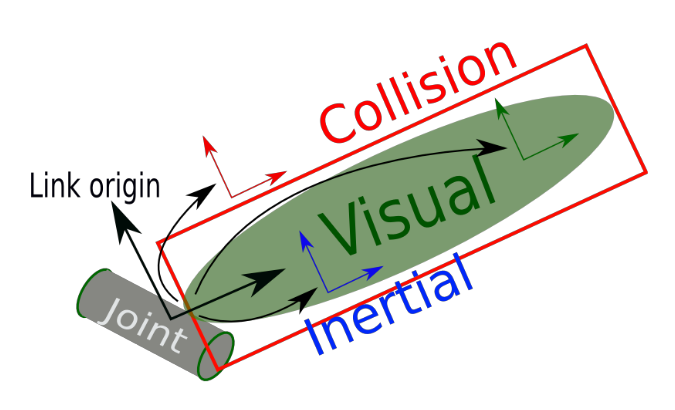
\includegraphics[width = 0.4\linewidth]{image/link标签.png}
\end{figure}

从图中可以看出,检测碰撞的link区域大于外观可视的区域,这就意味着只要有其他物体与collision区域相交,就认为link发生碰撞。

<link>标签的一般结构如下:

\begin{verbatim}
    <link name = "<name of the link>">
        <inertial> ...... </inertial>
        <visual> ...... </visual>
        <collision> ...... </collision>
    </link>
\end{verbatim}

其中:
\begin{itemize}
    \item <visual>:用于描述机器人link部分的外观参数
    \item <inertial>:用于描述link的惯性参数
    \item <collision>:用于描述link的碰撞部分
\end{itemize}

\subsection{<joint>标签}\label{subsec:joint}

<joint>标签用于描述机器人关节的运动学和动力学属性,包括关节运动的位置和速度限制。根据机器人的关节运动形式,可以将其分为六种类型:

\begin{table}[H]
    \centering
    \begin{tabular}{c|c}
    \hline
    \textbf{关节类型} & \textbf{描述}            \\ \hline
    continuous    & 旋转关节,可以围绕单轴无限旋转        \\ \hline
    revolute      & 旋转关节,有旋转的角度限制          \\ \hline
    prismatic     & 滑动关节,沿某一轴线移动的关节,带有位置极限 \\ \hline
    planar        & 平面关节,允许在平面正交方向上平移或者旋转  \\ \hline
    floating      & 浮动关节,允许进行平移、旋转运动       \\ \hline
    fixed         & 固定关节,不允许运动的特殊关节        \\ \hline
    \end{tabular}
\end{table}

机器人关节的主要作用是连接两个刚体link,这两个link分别称为parent link和child link,如下图所示:

\begin{figure}[H]
    \centering
    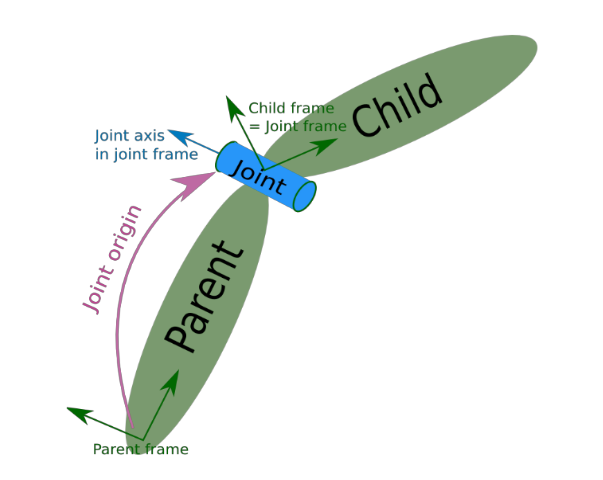
\includegraphics[width = 0.5\linewidth]{image/joint标签.png}
\end{figure}

<link>标签的一般结构如下:

\begin{verbatim}
    <joint name = "<name of the joint>">
        <parent link = "parent_link"/>
        <child link = "child_link"/>
        <calibration .... />
        <dynamics damping .... />
        <limit effort .... />
        ....
    </joint>
\end{verbatim}

其中必须指定joint的parent link和child link,还可以设置关节的其他属性:

\begin{itemize}
    \item <calibration>:关节的参考位置,用来校准关节的绝对位置。
    \item <dynamics>:用于描述关节的物理属性,例如阻尼、静摩擦力,经常在动力学仿真中出现。
    \item <limit>:用于描述运动的一些极限值,包括关节运动的上下限位置、速度限制、力矩限制等。
    \item <mimic>:用于描述该关节与已有关节的关系。
    \item <safety\_controller>:用于描述安全控制器参数。
\end{itemize}

\subsection{<robot>标签}

<robot>是完整机器人模型的最顶层标签,<link>和<joint>标签都必须包含在<robot>标签内。robot标签内可以设置机器人的名称,其基本语法如下:

\begin{verbatim}
    <robot name = "name of the robot">
        <link> ...... </link>
        <link> ...... </link>
        <joint> ...... </joint>
        <joint> ...... </joint>
    </robot>
\end{verbatim}

\subsection{<gazebo>标签}

<gazebo>标签用于描述机器人模型在Gazebo中仿真所需要的参数,包括机器人材料的属性、Gazebo插件。该标签不是机器人模型的必需部分,只有在Gazebo中仿真时才需要加入,其基本语法如下:

\begin{verbatim}
    <gazebo reference = "link_1">
        <material>Gazebo/Black</material>
    </gazebo>
\end{verbatim}

\section{创建URDF模型}

以MRobot机器人为例。

\subsection{创建功能包}

使用如下命令创建一个urdf模型的功能包:

\begin{verbatim}
    $ catkin_create_pkg mrobot_description urdf xacro
\end{verbatim}

创建好的功能包中包含如下四个文件夹:

\begin{itemize}
    \item urdf:用于存放机器人模型的URDF文件或xacro文件
    \item mashes:用于放置URDF中引用的模型渲染文件
    \item launch:用于保存相关启动文件
    \item config:用于保存rviz的配置文件
\end{itemize}

\subsection{URDF模型代码}

\subsubsection{part 1}

\begin{verbatim}
    <?xml version="1.0" ?>
    <robot name="mrobot_chassis">
\end{verbatim}

首先在文件开头,需要生命该文件使用XML描述,然后使用<robot>根标签定义一个机器人模型,并定义机器人的名称。

\subsubsection{part 2}
\begin{verbatim}
    <link name="base_link">
        <visual>
            <origin xyz=" 0 0 0" rpy="0 0 0" />
            <geometry>
                <cylinder length="0.005" radius="0.13"/>
            </geometry>
            <material name="yellow">
                <color rgba="1 0.4 0 1"/>
            </material>
        </visual>
    </link>
\end{verbatim}

这一段代码描述机器人的底盘link,<visual>标签定义底盘的外观属性;

在<geometry>标签下定义几何外观,我们将底盘抽象成一个圆柱,使用<cylinder>标签定义这个圆柱的半径和高;

然后声明这个底盘圆柱在三维坐标位置和旋转姿态,使用<origin>标签设置底盘中心位置,底盘中心位于界面的中心点,所以将坐标设置为“0 0 0”,旋转设置也设置为“0 0 0”即可(圆柱体默认是垂直地面放置的);

另外,使用<material>标签设置底盘的颜色——”黄色“,其中<color>标签定义颜色的RGBA值(这里采用百分数描述,A为透明度参数)。

\subsubsection{part 3}

\begin{verbatim}
    <joint name="base_left_motor_joint" type="fixed">
        <origin xyz="-0.055 0.075 0" rpy="0 0 0" />        
        <parent link="base_link"/>
        <child link="left_motor" />
    </joint>
\end{verbatim}

这一段代码定义一个关节joint,用来连接机器人底盘和左边驱动电机,joint类型为fixed类型,这种类型的joint是固定的(见\autoref{subsec:joint})。

<origin>标签设置了joint的起点,将起点设置在需要安装电机的底盘位置。

\subsubsection{part 4}

\begin{verbatim}
    <link name="left_motor">
        <visual>
            <origin xyz="0 0 0" rpy="1.5707 0 0" />
            <geometry>
                <cylinder radius="0.02" length = "0.08"/>
            </geometry>
            <material name="gray">
                <color rgba="0.75 0.75 0.75 1"/>
            </material>
        </visual>
    </link>
\end{verbatim}

这一段代码描述了左侧电机的模型,外形也是圆柱体,采用<cylinder>标签。

关于<origin>标签的设置:由于我们上面定义了一个joint用来将电机连接到底盘上,电机的位置是相对于joint计算的。在joint的位置设置中,已经将其放置到了安装电机的位置,所以电机模型的位置设置到“0 0 0”坐标就可以了。

另外由于圆柱体默认垂直地面,因此我们需要将电机模型绕x轴旋转90°放置。

\subsubsection{part 5}

\begin{verbatim}
    <joint name="left_wheel_joint" type="continuous">
        <origin xyz="0 0.0485 0" rpy="0 0 0"/>
        <parent link="left_motor"/>
        <child link="left_wheel_link"/>
        <axis xyz="0 1 0"/>
    </joint>
\end{verbatim}

这一段代码定义一个关节joint,用来连接电机和轮子,joint类型为continuous类型,这种类型的joint可以绕一个轴旋转(见\autoref{subsec:joint})。

<origin>标签将轮子的起点设置到电机的一端,<axis>标签定义该joint的旋转轴是y轴。

\subsubsection{添加物理和碰撞属性}

前面的代码仅创建了模型的可视化属性,还需要添加物理属性和碰撞属性,这里以机器人底盘base\_link为例:

\begin{verbatim}
    <link name="base_link">
        <intertial>
            <mass value="2"/>
            <origin xyz="0 0 0.0"/>
            <inertia ixx="0.01" ixy="0.0" ixz="0.0"
                     iyy="0.01" iyz="0.0" 
                     izz="0.5"/>
        </inertial>

        <visual>
            <origin xyz=" 0 0 0" rpy="0 0 0" />
            <geometry>
                <cylinder length="${base_link_length}" radius="${base_link_radius}"/>
            </geometry>
            <material name="yellow">
            </material>
        </visual>

        <collision>
            <origin xyz="0 0 0" rpy="0 0 0"/>
            <geometry>
                <cylinder length="${base_link_length}" radius="${base_link_radius}"/>
            </geometry>
        </collision>
    </link>
\end{verbatim}

其中<intertial>标签设置惯性参数,主要包括质量和惯性矩阵,如果是规则物体,可以通过尺寸、质量等公式计算得到惯性矩阵(这里有待学习补充)。

\section{使用xacro优化URDF模型}

URDF文件不支持代码复用的特性,因此针对URDF模型提出了一种精简化、可复用、模块化的描述形式——xacro。

xacro有两点优点:精简的模型代码、提供可编程接口。模型的后缀名由.urdf变为.xacro,并且需要在模型的<robot>标签中加入xacro的声明,代码如下:

\begin{verbatim}
    <?xml version="1.0"?>
    <robot name="mrobot" xmlns:xacro="http://www.ros.org/wiki/xacro">
\end{verbatim}

\subsection{xacro的三个机制}

\subsubsection{使用常量定义}

定义常量的语法如下:

\begin{verbatim}
    <xacro:property name="M_PI" value="3.14159"/>
\end{verbatim}

使用常量的语法如下:

\begin{verbatim}
    <origin xyz="0 0 0" rpy="${M_PI} 0 0"/>
\end{verbatim}

\subsubsection{调用数学公式}

在”\${}“语句中,不仅可以调用常量,还可以使用一些常用的数学运算,包括加减乘除、负号、括号等(所有运算都会被转换成浮点数进行),语法如下:

\begin{verbatim}
    <origin xyz="0 ${(motor_length+wheel_length)/2} 0" rpy="0 0 0"/>
\end{verbatim}

\subsubsection{使用宏定义}

xacro文件可以使用宏定义来声明重复使用的代码模块,而且可以包含输入参数,以MRobot机器人的八根支撑柱为例,宏定义的语法示例如下:

\begin{verbatim}
    <xacro:macro name="mrobot_standoff_2in" params="parent number x_loc y_loc z_loc">
        <joint name="standoff_2in_${number}_joint" type="fixed">
            <origin xyz="${x_loc} ${y_loc} ${z_loc}" rpy="0 0 0" />
            <parent link="${parent}"/>
            <child link="standoff_2in_${number}_link" />
        </joint>

        <link name="standoff_2in_${number}_link">
            <inertial>
                <mass value="0.001" />
                <origin xyz="0 0 0" />
                <inertia ixx="0.0001" ixy="0.0" ixz="0.0"
                         iyy="0.0001" iyz="0.0"
                         izz="0.0001" />
            </inertial>

            <visual>
                <origin xyz=" 0 0 0 " rpy="0 0 0" />
                <geometry>
                    <box size="0.01 0.01 0.07" />
                </geometry>
                <material name="black">
                    <color rgba="0.16 0.17 0.15 0.9"/>
                </material>
            </visual>

            <collision>
                <origin xyz="0.0 0.0 0.0" rpy="0 0 0" />
                <geometry>
                    <box size="0.01 0.01 0.07" />
                </geometry>
            </collision>
        </link>
    </xacro:macro>
\end{verbatim}

以上的宏定义包含五个输入参数:joint的parent link,支撑住的序号,支撑柱在xyz三个方向上的偏移。这个宏定义在定义一个支撑柱的时候,分别对其joint和link两个标签进行了定义。

当需要使用该宏模块的时候,按照如下语法进行调用:

\begin{verbatim}
    <mrobot_standoff_2in parent="base_link" number="1" x_loc="-${standoff_x/2 + 0.03}" 
y_loc="-${standoff_y - 0.03}" z_loc="${plate_height/2}"/>
\end{verbatim}


\subsection{引用xacro文件}

引用示例如下:

\begin{verbatim}
    <?xml version="1.0"?>
    <robot name="mrobot" xmlns:xacro="http://www.ros.org/wiki/xacro">
        <xacro:include filename="$(find mrobot_description)/urdf/mrobot_body.urdf
    .xacro" />
        <!-- MRobot机器人平台 -->
        <mrobot_body/>
    </robot>
\end{verbatim}

可以看到,在robot标签之间,首先使用了xacro:inlude标签,包含了另一个xacro模型文件,然后我们就可以在下面使用被包含文件中的模块了。接下来调用被包含文件中的机器人模型宏定义(机器人模型文件全部是在被包含文件中用一个宏来描述的)。

这样将整个机器人模型作为一个宏有什么好处呢?把机器人整体看做一个模块,方便与其他模型进行集成,比如在后续安装传感器等其他模块时。

\subsection{显示xacro优化后的模型}

\subsubsection{将xacro文件转化成URDF文件}

使用如下命令可以将xacro文件转换成URDF文件:

\begin{verbatim}
    $ rosrun xacro xacro.py mrobot.urdf.xacro > mrobot.urdf
\end{verbatim}

\subsubsection{直接调用xacro文件解析器}

也可以省略手动转换的过程,直接在启动文件中调用xacro解析器,自动将xacro转换成URDF文件,在launch文件中使用如下语句进行配置:

\begin{verbatim}
    <arg name="model" default="$(find xacro)/xacro --inorder '$(find mrobot_description)/urdf/mrobot.urdf.xacro'" />
	<arg name="gui" default="true" />
\end{verbatim}

进而可以直接使用这个修改后的启动文件,看到xacro格式的机器人模型。

\section{添加传感器模型}

首先我们需要自己创建一个传感器模型(xacro文件),或者去网上下载一个传感器的模型,这里以一个摄像头为例,其模型文件为camera.xacro。

进而我们可以创建一个顶层xacro文件,将机器人主体与摄像头连接起来:

\begin{verbatim}
    <?xml version="1.0"?>
    <robot name="mrobot" xmlns:xacro="http://www.ros.org/wiki/xacro">

        <xacro:include filename="$(find mrobot_description)/urdf/mrobot_body.urdf
    .xacro" />
        <xacro:include filename="$(find mrobot_description)/urdf/camera.xacro" />

        <xacro:property name="camera_offset_x" value="0.1" />
        <xacro:property name="camera_offset_y" value="0" />
        <xacro:property name="camera_offset_z" value="0.02" />

        <!-- MRobot机器人平台-->
        <mrobot_body/>

        <!-- Camera -->
        <joint name="camera_joint" type="fixed">
            <origin xyz="${camera_offset_x} ${camera_offset_y} ${camera_offset_z}" rpy="0 0 0" />
            <parent link="plate_2_link"/>
            <child link="camera_link"/>
        </joint>

        <xacro:usb_camera prefix="camera"/>

    </robot>
\end{verbatim}

在这个顶层文件中,包含了描述摄像头的模型文件以及描述机器人的模型文件,然后使用了一个fixed类型的joint把摄像头固定到机器人的指定位置。

\section{基于ArbotiX和rviz的仿真器}

ArbotiX提供一个差速控制器,通过接收速度控制指令更新机器人的joint状态,从而实现机器人在rviz中的运动。

\subsection{在ROS-melodic中安装ArbotiX}

Arbotix本质上就是一个功能包,我们需要像其他我们自己的功能包一样,将其放置在工作空间下的src目录下,直接从git上下载其源码:

\begin{verbatim}
    $ git clone -b indigo-devel https://github.com/vanadiumlabs/arbotix_ros.git
\end{verbatim}

然后重新编译工程即可(注意如果没有将设置环境变量的指令放到.bashrc中,在这里要记得使用source命令设置环境变量)。

\subsection{配置ArbotiX控制器}

我们只需要适当修改原本的launch文件,然后再创建一个控制器相关的配置文件就可以了。

\subsubsection{修改launch文件}

只是在显示机器人模型的launch文件的基础上加上如下内容:

\begin{verbatim}
    <node name="arbotix" pkg="arbotix_python" type="arbotix_driver" output="screen">
        <rosparam file="$(find mrobot_description)/config/fake_mrobot_arbotix.yaml" 
    command="load" />
        <param name="sim" value="true"/>
    </node>
\end{verbatim}

从以上代码可以看出,实际上就是添加了一个控制器节点,这里在仿真环境中使用,需要配置“sim”参数为true。另外,从这里可以看到,启动时还需要加载一个叫“fake\_mrobot\_arbotix.yaml”的配置文件。

\subsubsection{创建配置文件}

配置文件的目录为:功能包目录/config/下,文件内容如下:

\begin{verbatim}
    controllers: {
        base_controller: {
            type: diff_controller, 
            base_frame_id: base_footprint, 
            base_width: 0.26, 
            ticks_meter: 4100, 
            Kp: 12, 
            Kd: 12, 
            Ki: 0, 
            Ko: 50, 
            accel_limit: 1.0 
        }
    }
\end{verbatim}

控制器的名称为“base\_controller”,类型为“diff\_controller”(差速控制器),另外还给出了参考坐标系、底盘尺寸、PID参数等。

\subsection{运行仿真}

需要注意的是,我们要设置参考坐标系(fixed frame)为“odom”,才可以看到小车的移动。

\section{ros\_control}

ros\_control是一套机器人控制中间件,包含一系列控制器接口、传动装置接口、硬件接口、控制器工具箱等。

\subsection{ros\_control的框架}

\begin{figure}[H]
    \centering
    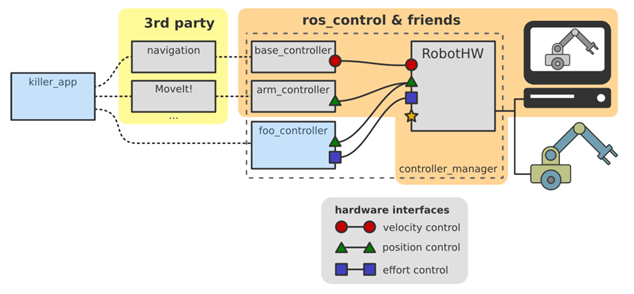
\includegraphics[width=0.8\linewidth]{image/ros_control.png}
\end{figure}

上图是ros\_control的总体框架,可以看到正对不同类型的控制器(底盘、机械臂等),ros\_control可以提供多种类型的控制器,但是这些控制器的接口各不相同,为了提高代码的复用率,ros\_control还提供一个硬件的抽象层。硬件抽象层负责机器人硬件资源的管理,而controller从抽象层请求资源即可,并不直接接触硬件。

\subsection{控制器}

ROS的ros\_controllers功能包提供了一些常用的控制器:

\begin{itemize}
    \item effort\_controllers
        \begin{itemize}
            \item joint\_effort\_controller
            \item joint\_position\_controller
            \item joint\_velocity\_controller
        \end{itemize}
    \item joint\_state\_controller
        \begin{itemize}
            \item joint\_state\_controller
        \end{itemize}
    \item position\_controllers
        \begin{itemize}
            \item joint\_position\_controller
        \end{itemize}
    \item velocity\_controllers
        \begin{itemize}
            \item joint\_velocity\_controller
        \end{itemize}
\end{itemize}

另外,也可以根据自己的需求创建需要的控制器,并通过控制器管理器进行管理(具体方法有需要再补充)。

\subsection{硬件接口}

\begin{figure}[H]
    \centering
    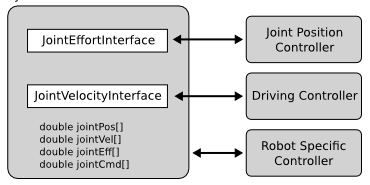
\includegraphics[width=0.4\linewidth]{image/硬件接口.png}
\end{figure}

硬件接口是控制器与RobotHW(硬件抽象层)沟通的接口,基本与控制器种类相对应。另外也可以根据自己的需求创建需要的接口(具体方法有需要再补充)。

\subsection{传动系统}

\subsection{关节约束}

\subsection{控制器管理器}

\section{Gazebo仿真}

\subsection{配置机器人模型}

首先我们需要确定每个link的<inertia>元素已经进行了合理的设置,然后还要为每个必要的<link>、<joint>、<robot>设置<gazebo>标签,进而我们需要为模型添加传动装置以及控制器插件。

\subsubsection{为link添加惯性参数和碰撞属性}

这个在前面URDF模型文件中已经提到过了,但是在rviz中这一项并不是必须的,其中的模型可以只有显示部分,并没有物理属性,但是gazebo中进行的是物理仿真,所以相关的惯性参数以及碰撞属性等物理参数就是必须的了。

另外,这里由于我们一般都使用xacro文件作为模型文件,相比URDF文件多了宏定义的机制;而且,我们知道,对于规则均匀刚体,其惯性参数矩阵是有一个固定的计算公式的。因此我们可以不再像之前那样每一个link的惯性参数都手动输入了,可以按照下面的方式采用宏定义进行自动计算,例如球体,我们可以定义这样一个宏用于计算其惯性矩阵:

\begin{verbatim}
    <xacro:macro name="sphere_inertial_matrix" params="m r">
        <inertial>
            <mass value="${m}" />
            <inertia ixx="${2*m*r*r/5}" ixy="0" ixz="0"
                    iyy="${2*m*r*r/5}" iyz="0" 
                    izz="${2*m*r*r/5}" />
        </inertial>
    </xacro:macro>
\end{verbatim}

类似地,长方体:

\begin{verbatim}
    <xacro:macro name="box_inertial_matrix" params="m w h d">
        <inertial>
            <mass value="${m}" />
            <inertia ixx="${m*(h*h+d*d)/12}" ixy = "0" ixz = "0"
                     iyy="${m*(w*w+d*d)/12}" iyz = "0"
                     izz="${m*(w*w+h*h)/12}" /> 
        </inertial>
    </xacro:macro>
\end{verbatim}

\subsubsection{为link添加<gazebo>标签}

需要为每一个link添加<gazebo>标签,包含的属性仅有material。注意:这里的material属性和<visual>中的material属性作用相同,但是Gazebo无法通过<visual>中的material属性设置外观颜色,因此需要再添加<gazebo>标签进行设置,另外,Gazebo中提供了一些可以直接使用的颜色供我们使用。

设置<gazebo>标签语法如下:

\begin{verbatim}
    <gazebo reference="wheel_${lr}_link">
        <material>Gazebo/Black</material>
    </gazebo>
\end{verbatim}

\subsubsection{为joint添加传动装置}

需要在模型中加入<transmission>元素,将传动装置与joint进行绑定。语法如下:

\begin{verbatim}
    <transmission name="wheel_${lr}_joint_trans">
        <type>transmission_interface/SimpleTransmission</type>
        <joint name="base_to_wheel_${lr}_joint" />
        <actuator name="wheel_${lr}_joint_motor">
            <hardwareInterface>VelocityJointInterface</hardwareInterface>
            <mechanicalReduction>1</mechanicalReduction>
        </actuator>
    </transmission>
\end{verbatim}

其中<type>标签声明了所使用的传动装置类型;<joint name>标签定义了将要绑定驱动器的joint;<actuator name>标签定义了传动装置的名称;并在其中使用<hardwareInterface>标签定义硬件接口类型,这里是速度控制接口;使用<mechanicalReduction>标签设置了传动比为1。

\subsubsection{添加Gazebo控制器插件}

Gazebo插件可以根据插件的运动范围应用到URDF模型的<robot>、<link>、<joint>上,需要使用<gazebo>标签作为封装,这里不同于上文中提到的“为link添加<gazebo>标签”,这里需要在<gazebo>标签下使用<plugin>标签来添加插件。

~\\
\noindent(1)为<link>、<joint>标签添加插件

设置reference为对应<link>或<joint>的名字,其中<plugin>标签下的插件名字name可以自拟,filename是gazebo提供的现成文件,可以查看ROS安装路径(/opt/ros/melodic/lib)下,所有插件都是以.so命名的。

\begin{verbatim}
    <gazebo reference="your_link_name">
        <plugin name="unique_name" filename="plugin_name.so"
            ...plugin parameters...
        </plugin>
    </gazebo>
\end{verbatim}

\noindent(2)为<robot>标签添加插件:

不设置reference属性即可。

\begin{verbatim}
    <gazebo>
        <plugin name="unique_name" filename="plugin_name.so"
            ...plugin parameters...
        </plugin>
    </gazebo>
\end{verbatim}

我们将一个差速控制的插件(libgazebo\_ros\_diff\_drive.so)应用到我们的示例机器人模型上,语法如下:

\begin{verbatim}
    <gazebo>
        <plugin name="differential_drive_controller" filename="libgazebo_ros_diff_drive.so">
            <rosDebugLevel>Debug</rosDebugLevel>
            <publishWheelTF>true</publishWheelTF>
            <robotNamespace>/</robotNamespace>
            <publishTf>1</publishTf>
            <publishWheelJointState>true</publishWheelJointState>
            <alwaysOn>true</alwaysOn>
            <updateRate>100.0</updateRate>
            <legacyMode>true</legacyMode>
            <leftJoint>base_to_wheel_left_joint</leftJoint>
            <rightJoint>base_to_wheel_right_joint</rightJoint>
            <wheelSeparation>${base_link_radius*2}</wheelSeparation>
            <wheelDiameter>${2*wheel_radius}</wheelDiameter>
            <broadcastTF>1</broadcastTF>
            <wheelTorque>30</wheelTorque>
            <wheelAcceleration>1.8</wheelAcceleration>
            <commandTopic>cmd_vel</commandTopic>
            <odometryFrame>odom</odometryFrame> 
            <odometryTopic>odom</odometryTopic> 
            <robotBaseFrame>base_footprint</robotBaseFrame>
        </plugin>
    </gazebo> 
\end{verbatim}

其中关键参数:
\begin{itemize}
    \item <robotNamespace>:机器人的命名空间,插件所有数据的发布和订阅都在该命名空间下。
    \item <leftJoint>和<rightJoint>:左右轮转动关节的joint,控制器插件最终需要控制这两个joint转动。
    \item <wheelSeparation>:轮子间距。
    \item <wheelDiameter>:轮子半径。
    \item \textcolor[rgb]{1,0,0}{wheelTorque>:这个怎么确定的?不重要吗?} 
    \item <wheelAcceleration>:车轮转动加速度。
    \item <commandTopic>:控制器订阅的速度控制指令,ROS中一般都命名为vel\_cmd。
    \item <odometryFrame>:里程计数据的参考坐标系,ROS中一般都命名为odom。
\end{itemize}

\subsection{显示机器人模型}

使用类似于以下的launch文件:

\begin{verbatim}
    <launch>
        <!-- 设置launch文件的参数 -->
        <arg name="world_name" value="$(find mrobot_gazebo)/worlds/playground.world"/>
        <arg name="paused" default="false"/>
        <arg name="use_sim_time" default="true"/>
        <arg name="gui" default="true"/>
        <arg name="headless" default="false"/>
        <arg name="debug" default="false"/>

        <!-- 运行gazebo仿真环境 -->
        <include file="$(find gazebo_ros)/launch/empty_world.launch">
            <arg name="world_name" value="$(arg world_name)" />
            <arg name="debug" value="$(arg debug)" />
            <arg name="gui" value="$(arg gui)" />
            <arg name="paused" value="$(arg paused)"/>
            <arg name="use_sim_time" value="$(arg use_sim_time)"/>
            <arg name="headless" value="$(arg headless)"/>
        </include>

        <!-- 加载机器人模型描述参数(模型的路径在这里) -->
        <param name="robot_description" command="$(find xacro)/xacro --inorder '$(
    find mrobot_gazebo)/urdf/mrobot.urdf.xacro'" /> 

        <!-- 运行joint_state_publisher节点,发布机器人的关节状态  -->
        <node name="joint_state_publisher" pkg="joint_state_publisher" type="joint_
    state_publisher" ></node> 

        <!-- 运行robot_state_publisher节点,发布tf  -->
        <node name="robot_state_publisher" pkg="robot_state_publisher" type="robot_
    state_publisher"  output="screen" >
            <param name="publish_frequency" type="double" value="50.0" />
        </node>

        <!-- 在gazebo中加载机器人模型-->
        <node name="urdf_spawner" pkg="gazebo_ros" type="spawn_model" respawn="false" 
    output="screen"
            args="-urdf -model mrobot -param robot_description"/> 
    </launch>
\end{verbatim}

当我们想要加载一个机器人模型到Gazebo中,都可以使用上面的这种launch文件的代码形式,主要需要修改的就是我们要加载的机器人模型的路径。

接下来,我们运行这个launch文件就可以启动Gazebo,并且在其中看到我们的机器人模型了。另外,由于这个模型已经订阅了vel\_cmd话题,我们也可以发布vel\_cmd话题消息来对Gazebo中的机器人进行控制了。

\subsection{摄像头仿真}

类似于机器人模型中的差速控制器插件,传感器的Gazebo插件也需要在URDF模型中进行配置,在原有的摄像头模型中添加<gazebo>标签,代码如下:

\begin{verbatim}
    <gazebo reference="${prefix}_link">
        <material>Gazebo/Black</material>
    </gazebo>

    <gazebo reference="${prefix}_link">
        <sensor type="camera" name="camera_node">
            <update_rate>30.0</update_rate>
            <camera name="head">
                <horizontal_fov>1.3962634</horizontal_fov>
                <image>
                    <width>1280</width>
                    <height>720</height>
                    <format>R8G8B8</format>
                </image>
                <clip>
                    <near>0.02</near>
                    <far>300</far>
                </clip>
                <noise>
                    <type>gaussian</type>
                    <mean>0.0</mean>
                    <stddev>0.007</stddev>
                </noise>
            </camera>
            <plugin name="gazebo_camera" filename="libgazebo_ros_camera.so">
                <alwaysOn>true</alwaysOn>
                <updateRate>0.0</updateRate>
                <cameraName>/camera</cameraName>
                <imageTopicName>image_raw</imageTopicName>
                <cameraInfoTopicName>camera_info</cameraInfoTopicName>
                <frameName>camera_link</frameName>
                <hackBaseline>0.07</hackBaseline>
                <distortionK1>0.0</distortionK1>
                <distortionK2>0.0</distortionK2>
                <distortionK3>0.0</distortionK3>
                <distortionT1>0.0</distortionT1>
                <distortionT2>0.0</distortionT2>
            </plugin>
        </sensor>
    </gazebo>
\end{verbatim}

这里添加了两个<gazebo>标签:

第一个<gazebo>标签用来设置摄像头模型在Gazebo中的material,与之前提到的为每一个link添加<gazebo>标签作用相同。

第二个<gazebo>标签设置摄像头插件。在加载摄像头插件的时候,需要使用<sensor>标签来包含传感器的各种属性。这里设置摄像头传感器,需要设置type为camera,传感器名字name可以自由设置;然后使用<camera>标签具体描述摄像头的参数,包括分辨率、编码格式、图像范围、噪声参数等;最后使用<plugin>标签加载摄像头的插件文件libgazebo\_ros\_camera.so,并设置插件的一下参数,包括命名空间、发布图像的话题、参考坐标系等。

启动Gazebo下的机器人仿真之后,输入如下命令,使用rqt工具来看到摄像头的图像:

\begin{verbatim}
    $ rqt_image_view
\end{verbatim}

注意需要选择合适的话题才可以正确查看。

\subsection{Kinect仿真}

添加如下<gazebo>标签:

\begin{verbatim}
    <gazebo reference="${prefix}_link">
        <sensor type="depth" name="${prefix}">
            <always_on>true</always_on>
            <update_rate>20.0</update_rate>
            <camera>
                <horizontal_fov>${60.0*M_PI/180.0}</horizontal_fov>
                <image>
                    <format>R8G8B8</format>
                    <width>640</width>
                    <height>480</height>
                </image>
                <clip>
                    <near>0.05</near>
                    <far>8.0</far>
                </clip>
            </camera>
            <plugin name="kinect_${prefix}_controller" filename="libgazebo_ros_openni
        _kinect.so">
                <cameraName>${prefix}</cameraName>
                <alwaysOn>true</alwaysOn>
                <updateRate>10</updateRate>
                <imageTopicName>rgb/image_raw</imageTopicName>
                <depthImageTopicName>depth/image_raw</depthImageTopicName>
                <pointCloudTopicName>depth/points</pointCloudTopicName>
                <cameraInfoTopicName>rgb/camera_info</cameraInfoTopicName>
                <depthImageCameraInfoTopicName>depth/camera_info</depthImageCameraIn
            foTopicName>
                <frameName>${prefix}_frame_optical</frameName>
                <baseline>0.1</baseline>
                <distortion_k1>0.0</distortion_k1>
                <distortion_k2>0.0</distortion_k2>
                <distortion_k3>0.0</distortion_k3>
                <distortiotinaji
    </gazebo>
\end{verbatim}

\textcolor[rgb]{1,0,0}{这里为什么不需要一个<gazebo>标签来设置摄像头模型在Gazebo中的material了?} 

这里需要设置传感器类型为depth,<camera>中的参数与摄像头的类似,分辨率和检测距离都可以在Kinect的手册中找到,最后使用<plugin>标签加载Kinect的插件文件libgazebo\_ros\_openni\_kinect.so,并设置插件相关参数。

启动Gazebo下的机器人仿真之后,输入如下命令,使用rviz来查看Kinect的点云数据:

\begin{verbatim}
    $ rosrun rivz rviz
\end{verbatim}

注意需要设置fixed frame为camera\_frame\_optical,并且添加一个PointCloud2插件,并设置插件的订阅话题为“/camera/depth/points”才可以正确查看。

\subsection{激光雷达仿真}

添加如下<gazebo>标签:

\begin{verbatim}
    <gazebo reference="${prefix}_link">
        <material>Gazebo/Black</material>
    </gazebo>

    <gazebo reference="${prefix}_link">
        <sensor type="ray" name="rplidar">
            <pose>0 0 0 0 0 0</pose>
            <visualize>false</visualize>
            <update_rate>5.5</update_rate>
            <ray>
                <scan>
                <horizontal>
                    <samples>360</samples>
                    <resolution>1</resolution>
                    <min_angle>-3</min_angle>
                    <max_angle>3</max_angle>
                </horizontal>
                </scan>
                <range>
                <min>0.10</min>
                <max>6.0</max>
                <resolution>0.01</resolution>
                </range>
                <noise>
                <type>gaussian</type>
                <mean>0.0</mean>
                <stddev>0.01</stddev>
                </noise>
            </ray>
            <plugin name="gazebo_rplidar" filename="libgazebo_ros_laser.so">
                <topicName>/scan</topicName>
                <frameName>laser_link</frameName>
            </plugin>
        </sensor>
    </gazebo>
\end{verbatim}

激光雷达的传感器类型为ray,rplidar的相关参数可以在产品手册中找到,<ray>标签中设置了如下的雷达参数:360°检测范围、单圈360个采样点、5.5Hz采样频率、最远6m检测范围等。最后使用<plugin>标签加载激光雷达的插件文件libgazebo\_ros\_laser.so,并设置插件相关参数。

启动Gazebo下的机器人仿真之后,输入如下命令,使用rviz来查看激光雷达的点云数据:

\begin{verbatim}
    $ rosrun rivz rviz
\end{verbatim}

注意需要设置fixed frame为base\_footprint,并且添加一个LaserScan插件,并设置插件的订阅话题为“/scan”才可以正确查看。

% -------------------------chapter 5-------------------------
\chapter{机器人SLAM与自主导航}

三个重点问题:地图的精确建模、机器人准确定位、路径实时规划。

\section{准备工作}

\subsection{机器人要求}

ROS中SLAM和自主导航的相关功能包可以用于各种移动机器人平台,但是为了达到最好的效果,对机器人硬件有如下的三个要求:

\begin{itemize}
    \item[-] 导航功能包对\textbf{差分、轮式机器人}的效果比较好,并且假设机器人可以直接使用速度指令进行控制,速度指令包括:linear(机器人在xyz三轴方向上的线速度,单位m/s);angular(机器人在xyz三轴方向上的角速度,单位是rad/s)。
    \item[-] 导航功能包要求机器人必须安装激光雷达等测距设备,可以获得环境的深度信息。
    \item[-] 导航功能包以正方形和圆形机器人为模板进行开发,对于其他外形的机器人,虽然可以使用,但是效果可能不佳。
\end{itemize}

\subsection{传感器信息}

\subsubsection{环境深度信息}

针对激光雷达,ROS在sensor\_msgs包中定义了专用的数据结构——LaserScan,用于存储激光消息,其消息的核心内容如下:

\begin{itemize}
    \item angle\_min:可检测范围的起始角度。
    \item angle\_max:可检测范围的终止角度,与angle\_min组成激光雷达的可检测范围。
    \item angle\_increment:采集到相邻数据帧之间的角度步长。
    \item time\_increment:采集到相邻数据帧之间的时间步长,\textcolor[rgb]{1,0,0}{当传感器处于相对运动状态时进行补偿使用。}
    \item scan\_time:采集一帧数据所需要的时间。
    \item range\_min:最近可检测深度的阈值。
    \item range\_max:最远可检测深度的阈值。
    \item ranges:一帧深度数据的存储数组。
\end{itemize}

如果使用的机器人没有激光雷达,但是配备有Kinect等RGB-D摄像头,也可以通过红外摄像头获取周围环境中的深度信息。但是RGB-D摄像头获取的原始深度信息是三维点云数据,我们需要将三维数据转换成二维数据,即只抽取其中的一行,重新封装为LaserScan消息,就可以获得需要的二维激光雷达信息。

ROS中也提供了相应的功能包——depthimage\_to\_laserscan来实现三维点云数据到二维的转换功能,从而将点云深度数据转换成激光数据。可以在launch文件中使用如下方法调用:

\begin{verbatim}
    <node pkg="depthimage_to_laserscan" type="depthimage_to_laserscan" name="depth
image_to_laserscan" output="screen">
        <remap from="image" to="/camera/depth_registered/image_raw"/> 
        <remap from="camera_info" to="/camera/depth_registered/camera_info"/>
        <remap from="scan" to="/kinect_scan"/>
        <param name="output_frame_id" value="/camera_link"/>
    </node>
\end{verbatim}

\subsubsection{里程计信息}

里程计根据传感器获取的数据来估计机器人随时间发生的位置变化,在机器人平台中,较为常见的里程计是编码器。里程计一般根据速度对时间的积分求得位置,这种方法对误差十分敏感,所以采取如精确的数据采集、设备标定、数据滤波等措施是十分必要的。

导航功能包要求机器人能够发布里程计nav\_msgs/Odometry消息,其中包含机器人在自由空间中的位置和速度的估算值:

\begin{itemize}
    \item pose:机器人当前位置坐标,包括机器人的xyz三轴位置与方向参数,以及用于校正误差的协方差矩阵。
    \item twist:机器人当前的运动状态,包括xyz三轴的线速度与角速度,以及用于校正误差的协方差矩阵。
\end{itemize}

\textcolor[rgb]{1,0,0}{上述数据结构中,用于滤波算法的协方差矩阵,在精度要求不高的机器人系统中可以使用默认的协方差矩阵;而在精度要求较高的系统中,需要先对机器人精确建模后,再通过仿真、实验等方法确定该矩阵的具体数值。}

\section{gmapping}

gmapping已经集成在ROS中,是移动机器人中使用最多的SLAM算法。这个算法是一种基于 Rao-Blackwellized的粒子滤波的 SLAM方法。基于粒子滤波的算法用许多加权粒子表示路径的后验概率,每个粒子都给出一个重要性因子。但是,它们通常需要大量的粒子才能获得比较好的的结果,从而增加该算法的的计算复杂性。

\subsection{gmapping功能包介绍}

\begin{figure}[H]
    \centering
    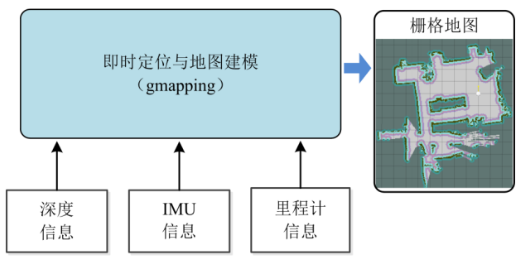
\includegraphics[width=0.5\linewidth]{image/gmapping框架.png}
\end{figure}

gmapping功能包订阅机器人的深度信息、IMU信息和里程计信息,同时完成一些必要参数的配置,即可创建并输出\textbf{基于概率}的二维栅格地图。

gmapping功能包向用户开放的接口如下:

(1)话题和服务:

\begin{table}[H]
    \centering
    \begin{tabular}{c|c|c|c}
    \hline
                                                                        & 名称            & 类型                      & 描述                                                                    \\ \hline
    \multirow{2}{*}{\begin{tabular}[c]{@{}c@{}}Topic\\ 订阅\end{tabular}} & tf            & tf/tfMessage            & \begin{tabular}[c]{@{}c@{}}用于激光雷达坐标系、基坐标系、\\ 里程计坐标系之间的变换\end{tabular} \\ \cline{2-4} 
                                                                        & scan          & sensor\_msgs/LaserScan  & 激光雷达扫描数据                                                              \\ \hline
    \multirow{3}{*}{\begin{tabular}[c]{@{}c@{}}Topic\\ 发布\end{tabular}} & map\_metadata & nav\_msgs/MapMetaData   & 发布地图Meta数据                                                            \\ \cline{2-4} 
                                                                        & map           & nav\_msgs/OccupancyGrid & 发布地图栅格数据                                                              \\ \cline{2-4} 
                                                                        & $\sim$entropy & std\_msgs/Float64       & 发布机器人姿态分布熵的估计                                                         \\ \hline
    Service                                                             & dynamic\_map  & nav\_msgs/GetMap        & 获取地图数据                                                                \\ \hline
    \end{tabular}
    \end{table}

(2)坐标变换:

\begin{table}[H]
    \centering
    \begin{tabular}{c|c|l}
        \hline
                                 & TF变换                                            & 描述                                                                                                                          \\ \hline
        \multirow{2}{*}{必需的TF变换} & \textless{}scan frame\textgreater $\rightarrow$ base\_link & \begin{tabular}[c]{@{}l@{}}激光雷达坐标系与基坐标系之间的变换,\\ 一般由robot\_states\_publisher或者\\ static\_transform\_publisher发布\end{tabular} \\ \cline{2-3} 
                                 & base\_link $\rightarrow$ odom                              & \begin{tabular}[c]{@{}l@{}}基坐标系与里程计坐标系之间的变换,\\一般由里程计节点发布\end{tabular}                                                      \\ \hline
        发布的TF变换                  & map $\rightarrow$ odom                                     & \begin{tabular}[c]{@{}l@{}}地图坐标系与机器人里程计坐标系之间的\\变换,估计机器人在地图中的位姿\end{tabular}                                                \\ \hline
        \end{tabular}
        \end{table}

(3)参数

gmapping功能包中可供配置的参数有很多,使用后将重点参数记录在下面:



\subsection{gmapping节点配置与运行}

首先创建一个运行gmapping节点的launch文件(gmapping.launch),主要用于节点参数的配置,文件代码如下:

\begin{verbatim}
    <launch>
        <arg name="scan_topic" default="scan" />

        <node pkg="gmapping" type="slam_gmapping" name="slam_gmapping" output="scr
    een" clear_params="true">
            <param name="odom_frame" value="odom"/>
            <param name="map_update_interval" value="5.0"/>
            <!-- Set maxUrange < actual maximum range of the Laser -->
            <param name="maxRange" value="5.0"/>
            <param name="maxUrange" value="4.5"/>
            <param name="sigma" value="0.05"/>
            <param name="kernelSize" value="1"/>
            <param name="lstep" value="0.05"/>
            <param name="astep" value="0.05"/>
            <param name="iterations" value="5"/>
            <param name="lsigma" value="0.075"/>
            <param name="ogain" value="3.0"/>
            <param name="lskip" value="0"/>
            <param name="srr" value="0.01"/>
            <param name="srt" value="0.02"/>
            <param name="str" value="0.01"/>
            <param name="stt" value="0.02"/>
            <param name="linearUpdate" value="0.5"/>
            <param name="angularUpdate" value="0.436"/>
            <param name="temporalUpdate" value="-1.0"/>
            <param name="resampleThreshold" value="0.5"/>
            <param name="particles" value="80"/>
            <param name="xmin" value="-1.0"/>
            <param name="ymin" value="-1.0"/>
            <param name="xmax" value="1.0"/>
            <param name="ymax" value="1.0"/>
            <param name="delta" value="0.05"/>
            <param name="llsamplerange" value="0.01"/>
            <param name="llsamplestep" value="0.01"/>
            <param name="lasamplerange" value="0.005"/>
            <param name="lasamplestep" value="0.005"/>
            <remap from="scan" to="$(arg scan_topic)"/>
        </node>
    </launch>
\end{verbatim}

这些参数都有默认值,可以等SLAM可以正常运行之后,再考虑调整优化参数。但是需要重点检查这两个参数:

\begin{itemize}
    \item 里程计坐标系的设置,odom\_frame参数需要和机器人本身的里程计坐标系一致。
    \item 激光雷达的话题名,gmapping节点订阅的激光雷达话题名是“/scan”,如果与机器人发布的激光雷达话题名不一致,需要使用<remap>进行重映射。
\end{itemize}

接下来创建一个启动gmapping例程的文件(gmapping\_demo.launch)。主要代码如下:

\begin{verbatim}
    <launch>
        <include file="$(find mrobot_navigation)/launch/gmapping.launch"/>
        <!-- 启动rviz -->
        <node pkg="rviz" type="rviz" name="rviz" args="-d $(find mrobot_navigation)/rviz/gmapping.rviz"/>
    </launch>
\end{verbatim}

这个launch文件主要包含:

\begin{itemize}
    \item 启动之前创建的gmapping节点。
    \item 启动rviz界面,查看传感器和地图构建的实时信息。
\end{itemize}

\subsection{在Gazebo中仿真SLAM(gmapping)}

启动Gazebo仿真环境和gmapping节点:

\begin{verbatim}
    $ roslaunch mrobot_gazebo mrobot_laser_nav_gazebo.launch
    $ roslaunch mrobot_navigation gmapping_demo.launch
\end{verbatim}

启动键盘控制节点:

\begin{verbatim}
    $ roslaunch mrobot_teleop mrobot_teleop.launch
\end{verbatim}

操作机器人在地图中运动一圈,就可以基本完成地图的构建了,构建完成后,可以使用如下命令保存构建好的地图:

\begin{verbatim}
    $ rosrun map_server map_saver
\end{verbatim}

保存好的文件默认文件名为map,包含:
\begin{itemize}
    \item 一个map.pgm地图数据文件
    \item 一个map.yaml地图配置文件:其中包含关联的地图数据文件、地图分辨率、起始位置、地图数据和阈值等配置参数。
\end{itemize}

\section{hector-slam}

hector\_slam功能包使用高斯牛顿法,不需要里程计数据,只根据激光信息便可构建地图。因此该功能包可以很好的在空中机器人、手持构图设备以及特种机器人中使用。但是该算法需要高更新频率小测量噪声的激光雷达,当只有低更新率的激光传感器时,即便测距估计很精确,对该系统都会出现一定的问题。

\section{cartographer}

cartographer是Google的实时室内建图项目,考虑到基于模拟策略的粒子滤波方法在较大环境中对内存和计算资源的需求较高,cartographer采用基于图网络的优化方法。

\section{rgbdslam}

不同于上述方法,rgbdslam是一个3D SLAM功能包。可以实现三维信息的地图构建,可以把周围环境的三维模型全部构建出来,机器人不仅知道地图中的什么位置有一个障碍物,而且知道该障碍物是什么。

\section{ORB\_SLAM}

ORB\_SLAM是一个基于特征点的实时单目SLAM系统,能够实时解算摄像机的移动轨迹,同时构建简单的三维点云地图,在大范围中做闭环检测,并实时进行全局重定位,不仅适用于手持设备获取的一组连续图像,同时适用于汽车行驶过程中获取的连续图像。

\section{导航功能包}

\subsection{导航框架}

导航的关键是机器人的定位和路径规划两大部分,ROS也对应地提供了两个功能包:

\begin{itemize}
    \item move\_base:实现机器人导航中的最优路径规划。
    \item amcl:实现二维地图中的机器人定位。
\end{itemize}

在上述两个功能包的基础上,ROS提供了一整套导航功能框架,如下图所示:

\begin{figure}[H]
    \centering
    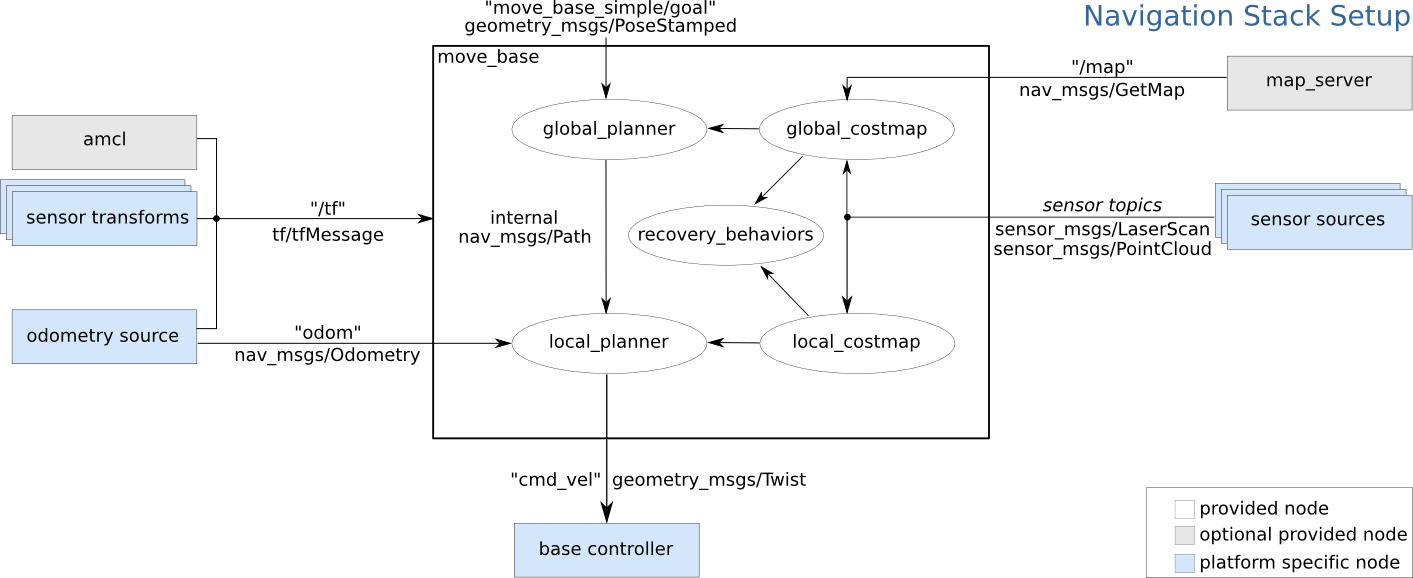
\includegraphics[width=1.0\linewidth]{image/导航功能包框架.png}
\end{figure}

机器人需要发布必要的传感器信息和导航的目标位置;move\_base功能包提供导航的主要运行、交互接口;amsl功能包对机器人进行精确定位,保障导航路径的准确性。

机器人通过ROS发布sensor\_msgs/LaserScan或者sensor\_msgs/PointCloud格式的消息,也就是二维激光信息或者三维点云信息,从而为导航功能包提供机器人的传感器信息,以达到实时避障的效果。

其次导航包要求机器人发布nav\_msgs/Odometry格式的里程计信息,同时也要发布相应的TF变换。

最后导航功能包的输出是geometry\_msgs/Twist格式的控制指令,这就要求机器人控制节点具备解析控制指令中线速度、角速度的能力,并且最终通过这些指令控制机器人完成相应的运动。

\subsection{move\_base功能包}

move\_base功能包中主要由两个规划器组成:

\begin{itemize}
    \item 全局路径规划(global\_planner):根据给定的目标位置和全局地图进行总体的路径规划(使用Dijkstra或者$A^{*}$算法)。
    \item 本地路径规划(local\_planner): 针对地图信息和机器人附近随时可能出现的障碍物规划机器人每个周期内应该行使的路径。使之尽可能符合全局最优路径(使用Dynamic Window Approaches算法搜索躲避和行进的多条路径,综合各评价标准(是否会撞击障碍物、所需要的时间)选取最优路径,并且计算行使周期内的线速度和角速度,避免与动态出现的障碍物发生碰撞)。
\end{itemize}

move\_base功能包的一些接口:

(1)话题和服务

\begin{table}[H]
    \centering
    \begin{tabular}{c|c|c|l}
        \hline
                                                                         & 名称                                                                    & 类型                                                                                 & \multicolumn{1}{c}{描述}                                                                             \\ \hline
        \multirow{2}{*}{\begin{tabular}[c]{@{}c@{}}动作\\ 订阅\end{tabular}} & \begin{tabular}[c]{@{}c@{}}move\_base/\\ goal\end{tabular}            & \begin{tabular}[c]{@{}c@{}}move\_base\_msgs/\\ MoveBaseActionGoal\end{tabular}     & move\_base的运动规划目标                                                                                  \\ \cline{2-4} 
                                                                         & \begin{tabular}[c]{@{}c@{}}move\_base/\\ cancel\end{tabular}          & actionlib\_msgs/GoalID                                                             & 取消特定目标的请求                                                                                          \\ \hline
        \multirow{3}{*}{\begin{tabular}[c]{@{}c@{}}动作\\ 发布\end{tabular}} & \begin{tabular}[c]{@{}c@{}}move\_base/\\ feedbback\end{tabular}       & \begin{tabular}[c]{@{}c@{}}move\_base\_msgs/\\ MoveBaseActionFeedback\end{tabular} & \begin{tabular}[c]{@{}l@{}}反馈信息\\ 含有机器人底盘的坐标\end{tabular}                                          \\ \cline{2-4} 
                                                                         & \begin{tabular}[c]{@{}c@{}}move\_base/\\ status\end{tabular}          & \begin{tabular}[c]{@{}c@{}}actionlib\_msgs/\\ GoalStatusArray\end{tabular}         & 发送到move\_base的目标状态信息                                                                               \\ \cline{2-4} 
                                                                         & \begin{tabular}[c]{@{}c@{}}move\_base/\\ result\end{tabular}          & \begin{tabular}[c]{@{}c@{}}move\_base\_msgs/\\ MoveBaseActionResult\end{tabular}   & 此处move\_base操作结果为空                                                                                 \\ \hline
        \begin{tabular}[c]{@{}c@{}}话题\\ 订阅\end{tabular}                  & \begin{tabular}[c]{@{}c@{}}move\_base\_\\ simple/goal\end{tabular}    & \begin{tabular}[c]{@{}c@{}}geometry\_msgs/\\ PoseStamped\end{tabular}              & \begin{tabular}[c]{@{}l@{}}为无需追踪目标执行状态的用户\\ 提供一个非action接口\end{tabular}                             \\ \hline
        \begin{tabular}[c]{@{}c@{}}话题\\ 发布\end{tabular}                  & cmd\_vel                                                              & geometry\_msgs/Twist                                                               & 输出到机器人底盘的速度指令                                                                                      \\ \hline
        \multirow{3}{*}{服务}                                              & $\sim$make\_plan                                                      & nav\_msgs/GetPlan                                                                  & \begin{tabular}[c]{@{}l@{}}允许用户从move\_base获取给定目标\\ 的路径规划,但不会执行该路径规划\end{tabular}                   \\ \cline{2-4} 
                                                                         & \begin{tabular}[c]{@{}c@{}}$\sim$clean\_unknow\\ \_space\end{tabular} & std\_srvs/Empty                                                                    & \begin{tabular}[c]{@{}l@{}}允许用户直接清除机器人周围的未知\\ 空间,适合costmap停止很长时间之后 \\ 在一个全新环境中重新启动时使用\end{tabular} \\ \cline{2-4} 
                                                                         & $\sim$clear\_costmaps                                                 & std\_srvs/Empty                                                                    & \begin{tabular}[c]{@{}l@{}}允许用户命令move\_base节点清除\\ costmap中的障碍,这可能会导致\\ 机器人撞上障碍物,谨慎使用\end{tabular}  \\ \hline
    \end{tabular}
\end{table}

(2)参数

待补充

\subsection{amcl功能包}

自主定位即机器人在任意状态下都可以推算出自己在地图中所处的位置。ROS为开发者提供了一种自适应(或kld采样)的蒙特卡洛定位方法(amcl),这是一种概率统计方法,针对已有地图使用粒子滤波器跟踪一个机器人的姿态。

amcl功能包的一些接口:

(1)话题和服务

\begin{table}[H]
    \centering
    \begin{tabular}{c|c|c|l}
        \hline
                                                                         & 名称                                                                   & 类型                                                                                  & \multicolumn{1}{c}{描述}                                                                       \\ \hline
        \multirow{4}{*}{\begin{tabular}[c]{@{}c@{}}话题\\ 订阅\end{tabular}} & Scan                                                                 & sensor\_msgs/LaserScan                                                              & 激光雷达数据                                                                                       \\ \cline{2-4} 
                                                                         & Tf                                                                   & tf/tfMessgae                                                                        & 坐标变换信息                                                                                       \\ \cline{2-4} 
                                                                         & initialpose                                                          & \begin{tabular}[c]{@{}c@{}}geometry\_msgs/\\ PoseWithCovarianceStamped\end{tabular} & \begin{tabular}[c]{@{}l@{}}用来初始化粒子滤波器的均\\ 值和协方差\end{tabular}                                 \\ \cline{2-4} 
                                                                         & map                                                                  & nav\_msgs/OccupancyGrid                                                             & \begin{tabular}[c]{@{}l@{}}设置use\_map\_topic参数时\\ ,amcl订阅map话题以获取\\ 地图数据,用于激光定位\end{tabular} \\ \hline
        \multirow{3}{*}{\begin{tabular}[c]{@{}c@{}}话题\\ 发布\end{tabular}} & amcl\_pose                                                           & \begin{tabular}[c]{@{}c@{}}geometry\_msgs/\\ PoseWithCovarianceStamped\end{tabular} & \begin{tabular}[c]{@{}l@{}}机器人在地图中的位姿估计,\\ 带有协方差信息\end{tabular}                              \\ \cline{2-4} 
                                                                         & particlecloud                                                        & geometry\_msgs/PoseArray                                                            & \begin{tabular}[c]{@{}l@{}}粒子滤波器维护的位姿估计\\ 集合\end{tabular}                                    \\ \cline{2-4} 
                                                                         & Tf                                                                   & tf/tfMessgae                                                                        & 发布从odom到map的转换                                                                               \\ \hline
        \multirow{2}{*}{服务}                                              & global\_lacalization                                                 & std\_srvs/Empty                                                                     & \begin{tabular}[c]{@{}l@{}}初始化全局定位,所有粒子\\ 被随机撒在地图的空闲区域\end{tabular}                          \\ \cline{2-4} 
                                                                         & \begin{tabular}[c]{@{}c@{}}request\_nomotion\\ \_update\end{tabular} & std\_srvs/Empty                                                                     & \begin{tabular}[c]{@{}l@{}}手动执行更新并发布更新的\\ 粒子\end{tabular}                                    \\ \hline
        \begin{tabular}[c]{@{}c@{}}服务\\ 调用\end{tabular}                  & static\_map                                                          & nav\_msgs/GetMap                                                                    & \begin{tabular}[c]{@{}l@{}}amcl调用该服务来获取地图\\ 数据\end{tabular}                                  \\ \hline
        \end{tabular}
        \end{table}
(2)参数

待补充

(3)坐标变换

\begin{figure}[H]
    \centering
    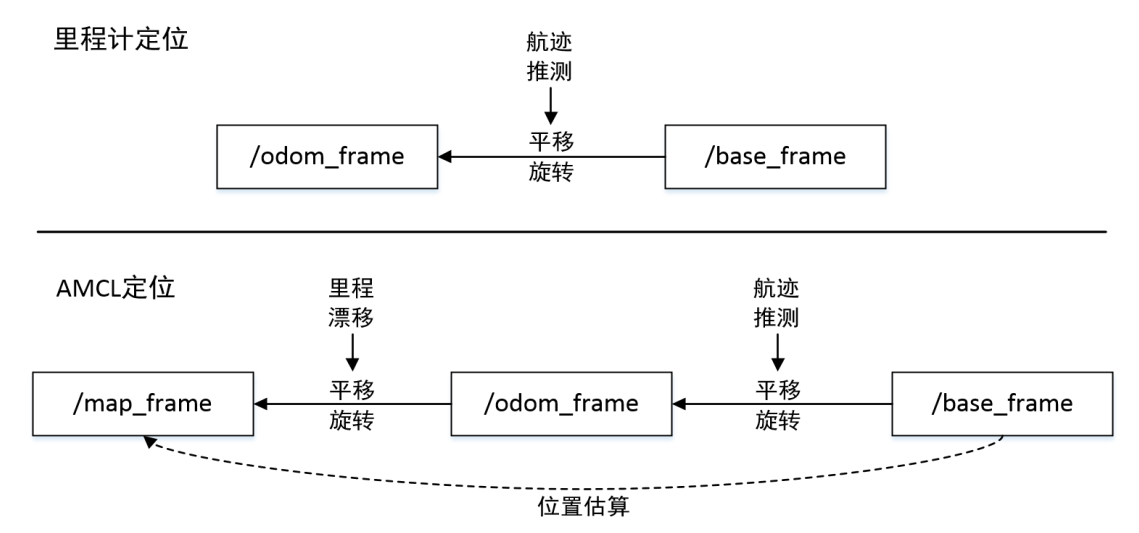
\includegraphics[width=0.8\linewidth]{image/amcl坐标变换.png}
\end{figure}

里程计定位和amcl定位的区别:

\begin{itemize}
    \item 里程计定位:只是通过里程计的数据来处理/base和/odom之间的TF变换
    \item amcl定位:可以估算机器人在地图坐标系/map下的位姿信息,提供/base、/odom、/map之间的TF变换。
\end{itemize}

\subsection{代价地图的配置}

\textcolor[rgb]{1,0,0}{代价地图的名称的意义是什么?}

导航功能包使用两种代价地图存储周围环境中的障碍信息:一种用于全局路径规划(global\_costmap),一种用于本地路径规划和实时避障(lacal\_costmap)。

两种代价地图需要使用共用的配置文件:通用配置文件;以及分别独立的配置文件:全局规划配置文件和本地规划配置文件。

\subsubsection{通用配置文件}

代价地图用来存储周围环境的障碍信息,其中需要声明地图专注的机器人传感器信息,以便于地图信息的更新。对于两种代价地图通用的配置选项,创建一个名为costmap\_common\_params.yaml的配置文件,代码如下:

\begin{verbatim}
    obstacle_range: 2.5
    raytrace_range: 3.0
    # footprint: [[0.175, 0.175], [0.175, -0.175], [-0.175, -0.175], [-0.175, 0.175]]
    # footprint_inflation: 0.01
    robot_radius: 0.175
    inflation_radius: 0.15
    max_obstacle_height: 0.6
    min_obstacle_height: 0.0
    observation_sources: scan
    scan: {data_type: LaserScan, topic: /scan, marking: true, clearing: true, expec
ted_update_rate: 0}
\end{verbatim}

其中代码段:

\begin{verbatim}
    obstacle_range: 2.5
    raytrace_range: 3.0
\end{verbatim}

用来设置代价地图中障碍物的相关阈值:obstacle\_range参数用来设置机器人检测障碍物的最大范围,若设置为2.5,则表示在2.5m范围内检测道德障碍物信息才会在地图中进行更新;raytrace\_range参数用来设置机器人检测自由空间的最大范围,若设置为3.0,则表示在3m范围内,机器人将根据传感器信息清除范围内的自由空间\textcolor[rgb]{1,0,0}{(这里的自由空间是不是指没有障碍物的空间)}。

代码段:

\begin{verbatim}
    # footprint: [[0.175, 0.175], [0.175, -0.175], [-0.175, -0.175], [-0.175, 0.175]]
    # footprint_inflation: 0.01
    robot_radius: 0.175
    inflation_radius: 0.1
\end{verbatim}

footprint参数用来设置机器人在二维地图上占用的面积,参数以机器人的中心作为坐标原点。如果机器人的外形是圆形的,则需要设置机器人的外形半径robot\_radius。inflation\_radius参数用来设置障碍物的膨胀系数,也就是机器人应该与障碍物保持的最小安全距离,这里设置为0.1,表示机器人规划的路径应该与障碍物保持0.1m以上的安全距离。

代码段:

\begin{verbatim}
    max_obstacle_height: 0.6
    min_obstacle_height: 0.0
\end{verbatim}

这两个参数用来描述障碍物的最大高度和最小高度。(\textcolor[rgb]{1,0,0}{有什么用呢?})

代码段:

\begin{verbatim}
    observation_sources: scan
    scan: {data_type: LaserScan, topic: /scan, marking: true, clearing: true, expec
ted_update_rate: 0}
\end{verbatim}

observation\_sources参数列出了代价地图需要关注的所有传感器信息,每个传感器信息都会在后面列举出详细内容。

这里以激光雷达为例:

\begin{itemize}
    \item sensor\_farme表示传感器的参考系名称;
    \item data\_type表示激光数据或者点云数据使用的消息类型;
    \item topic\_name表示传感器发布的话题名称;
    \item marking和clearing表示是否需要使用传感器的实时信息来添加或者清除代价函数中的障碍物信息。
\end{itemize}

\subsubsection{全局规划配置文件}

全局规划配置文件用来存储全局代价地图的配置参数,命名为global\_costmap\_params.yaml,代码如下:

\begin{verbatim}
    global_costmap:
        global_frame: map
        robot_base_frame: base_footprint
        update_frequency: 1.0
        publish_frequency: 1.0
        static_map: true
        rolling_window: false
        resolution: 0.01
        transform_tolerance: 1.0
        map_type: costmap
 \end{verbatim}

\begin{itemize}
    \item global\_frame参数用来表示全局代价函数需要在哪个参考系下匀性,这里选择了map参考系;
    \item robot\_base\_frame参数用来设置代价地图可以参考的机器人本体的坐标系;
    \item update\_frequency参数决定全局地图信息更新的频率;
    \item static\_map参数用来决定代价地图是否需要根据map\_server提供的地图信息进行初始化。
\end{itemize}

\subsubsection{本地规划配置文件}

本地规划配置文件用来存储本地代价地图的配置参数,命名为local\_costmap\_params.yaml,代码如下:

\begin{verbatim}
    local_costmap:
        global_frame: odom
        robot_base_frame: base_footprint
        update_frequency: 3.0
        publish_frequency: 1.0
        static_map: true
        rolling_window: false
        width: 6.0
        height: 6.0
        resolution: 0.01
        transform_tolerance: 1.0
\end{verbatim}

前面几个参数的意义与全局规划配置文件相同,另外:

\begin{itemize}
    \item publish\_frequency参数用来设置代价地图发布可视化信息的频率;
    \item rolling\_window参数用来设置在机器人移动过程中是否需要滚动窗口,以保持机器人在中心;
    \item width、height、resolution参数设置代价地图的长、高、分辨率(米/格)。
\end{itemize}

\subsection{本地规划器配置}

本地规划器的主要作用为:根据规划的全局路径计算发布给机器人的速度控制指令。该规划器要根据机器人的规格配置相关参数,创建名为base\_local\_planner\_params.yaml的配置文件,代码如下:

\begin{verbatim}
    controller_frequency: 3.0
    recovery_behavior_enabled: false
    clearing_rotation_allowed: false

    TrajectoryPlannerROS:
        max_vel_x: 0.5
        min_vel_x: 0.1
        max_vel_y: 0.0  # zero for a differential drive robot
        min_vel_y: 0.0
        max_vel_theta: 1.0
        min_vel_theta: -1.0
        min_in_place_vel_theta: 0.5
        escape_vel: -0.1
        acc_lim_x: 1.5
        acc_lim_y: 0.0 # zero for a differential drive robot
        acc_lim_theta: 1.2

        holonomic_robot: false
        yaw_goal_tolerance: 0.1 # about 6 degrees
        xy_goal_tolerance: 0.1  # 10 cm
        latch_xy_goal_tolerance: false
        pdist_scale: 0.9
        gdist_scale: 0.6
        meter_scoring: true

        heading_lookahead: 0.325
        heading_scoring: false
        heading_scoring_timestep: 0.8
        occdist_scale: 0.1
        oscillation_reset_dist: 0.05
        publish_cost_grid_pc: false
        prune_plan: true

        sim_time: 1.0
        sim_granularity: 0.025
        angular_sim_granularity: 0.025
        vx_samples: 8
        vy_samples: 0 # zero for a differential drive robot
        vtheta_samples: 20
        dwa: true
        simple_attractor: false
\end{verbatim}

该配置文件中,声明机器人本地规划采用Trajectory Rollout算法,并设置算法中需要用到的机器人速度、加速度的阈值等参数。

\chapter{Navigation详细学习}

\section{三维空间中的刚体运动(基础知识补充)}

为什么要研究这个问题?因为当我们描述机器人的位姿时,就是在描述一个刚体在三维空间中的运动。

三维空间中,刚体的运动可以用两个概念来表示:旋转和平移。平移比较简单一些,一般用一个表示位移的向量来表示。而旋转则有多种表示方法,例如旋转矩阵、旋转向量等等,不同的表示方法各有优劣

\subsection{向量}

在描述旋转矩阵前我们先明确向量这个概念。向量是空间中的一个具体实物且不和任何实数相关联。为了描述向量,应该先确定一个具体的坐标系,明确该坐标系的线性基 $\begin{bmatrix} e_1 & e_2 & e_3 \end{bmatrix}$ 后才能够确定一个向量 $a$ 在该坐标系下的坐标:

\begin{equation}
    a = 
    \begin{bmatrix}
      e_1 & e_2 & e_3
    \end{bmatrix}
    \begin{bmatrix}
     a_1\\
     a_2\\
     a_3
    \end{bmatrix}
    = a_1e_1+a_2e_2+a_3e_3
\end{equation}

也就是说:向量坐标的具体取值,和向量本身和选取的坐标系相关。

接下来介绍向量间的两种运算:内积(点乘)和外积(叉乘)

内积可以描述向量之间的投影关系:

\begin{equation}
    a \cdot b = a^Tb = \sum_{i=1}^3 a_ib_i = |a||b|cos<a,b>
\end{equation}

外积可以表示向量的旋转:

\begin{equation}
    a \times b 
    = 
    \begin{vmatrix}
        i & j & k\\
        a_1 & a_2 & a_3\\
        b_1 & b_2 & b_3
    \end{vmatrix}
    =
    \begin{bmatrix}
        a_2b_3-a_3b_2\\
        a_3b_1-a_1b_3\\
        a_1b_2-a_1b_1
    \end{bmatrix}
    =
    \begin{bmatrix}
        0 & -a_3 & a_2\\
        a_3 & 0 & -a_1\\
        -a_2 & a_1 & 0
    \end{bmatrix}b
    =
    a^{\wedge}b
\end{equation}

外积的方向垂直于这两个向量,大小为$ |a||b|sin<a,b> $,是两个向量张成的四边形的有向面积。

其中我们引入了一个符号:$\wedge$,把$a$写成一个反对称矩阵,可以将其记成一个反对称符号。因此我们就把外积$a\times b$写成了矩阵和向量的乘法$a^{\wedge}b$,从而将其变成了线性运算。

用外积表示旋转:

在右手法则下,用右手的四个手指(握拳)从a转向b,大拇指的朝向就是旋转向量的方向,也就是$a\times b$的方向,它的大小由a和b的夹角决定。

\subsection{欧式变换}

假设存在两个坐标系:一个世界坐标系,是一个惯性系,认为它是固定不动的;另一个是一个机器人坐标系,是随机器人移动的坐标系。假设机器人观察到了某个向量$p$, 它在这两个坐标系中分别有一套坐标。前面说了,向量是一个客观存在的实体,那么必然有一个关系能够将这两套坐标联系起来。

这个关系就是欧式变换。因为机器人的运动是一个刚体运动,所以同一个向量在不同坐标系下的模长和方向都不会发生变化。这样一个欧式变换就是由一个旋转和一个平移两部分组成。

\subsection{旋转矩阵}

我们先考虑欧式变换中的旋转变换:

我们设某个单位正交基$(e_1,e_2,e_3)$,经过一次旋转之后,变成了$(e_1^\prime,e_2^\prime,e_3^\prime)$,那么对于同一个向量$a$,在两个坐标系下有不同的坐标:

\begin{equation}
    \begin{bmatrix}
        e_1 & e_2 & e_3
       \end{bmatrix}
       \begin{bmatrix}
        a_1\\
        a_2\\
        a_3
       \end{bmatrix}
       =
       \begin{bmatrix}
        e_1^\prime & e_2^\prime  & e_3^\prime 
       \end{bmatrix}
       \begin{bmatrix}
        a_1^\prime \\
        a_2^\prime \\
        a_3^\prime 
        \end{bmatrix}
\end{equation}

等式两边同时左乘$\begin{bmatrix}
    e_1^T\\
    e_2^T\\
    e_3^T
   \end{bmatrix}$,则左边的系数变成了单位阵,因此得到了两个坐标系的旋转关系:

\begin{equation}
    \begin{bmatrix}
        a_1\\
        a_2\\
        a_3
       \end{bmatrix}
       =
       \begin{bmatrix}
        e_1^Te_1^\prime & e_1^Te_2^\prime & e_1^Te_3^\prime\\
        e_2^Te_1^\prime & e_2^Te_2^\prime & e_2^Te_3^\prime\\
        e_3^Te_1^\prime & e_2^Te_2^\prime & e_3^Te_3^\prime
       \end{bmatrix}
       \begin{bmatrix}
        a_1\prime \\
        a_2\prime \\
        a_3\prime 
       \end{bmatrix}
       =
       Ra^\prime 
\end{equation}

我们把中间的矩阵拿出来,定义成一个矩阵 $R$ ,它描述了旋转本身,又称为旋转矩阵,是由两组基之间的内积组成的。而且它是一个行列式为1的正交矩阵(矩阵的转置等于矩阵的逆)。它的逆(亦即转置)描述了一个相反的的旋转。

接下来,加入欧式变换中的平移部分:

平移可以简单地用一个平移向量 $t$ 来表示,则欧式变换后的坐标为:

\begin{equation}
    a^\prime = Ra + t
\end{equation}

因此我们可以用一个旋转矩阵$R$和一个平移向量$t$完整地描述一个欧氏空间地坐标变换。

\subsection{变换矩阵与齐次坐标}

上面我们已经可以完整地表达欧氏空间地旋转和平移了,但是这里的变换并不是线性的,如果进行两次变换,则会得到下面的结果:

\begin{equation}
    c = R_2(R_1a+t_1)+t_2
\end{equation}

这样的形式在变换多次之后会变得非常复杂,因此我们需要引入齐次坐标,并将变换矩阵重写为:

\begin{equation}
    \begin{bmatrix}
        a^\prime \\
        1
       \end{bmatrix}
       =
       \begin{bmatrix}
        R & t\\
        0^T & 1
       \end{bmatrix}
       \begin{bmatrix}
        a\\
        1
       \end{bmatrix}
       =
       T
       \begin{bmatrix}
        a\\
        1
       \end{bmatrix}
\end{equation}

这里的矩阵T我们称为变换矩阵。

这其实是一个数学的技巧:我们在一个三维向量的末尾添加一个1,将其变为四维向量,称为齐次变换。对于四维向量,我们可以把旋转和平移写在一个变换矩阵中,从而使得整个关系变为线性关系。

变换矩阵的反向变换:

\begin{equation}
    T^{-1} =
    \begin{bmatrix}
        R^T & -R^Tt\\
        0^T & 1
    \end{bmatrix}
\end{equation}

\subsection{旋转向量}

我们容易想到,一个旋转只有三个自由度,一个三维刚体运动(包括旋转和平移)有六个自由度,但是对应的旋转矩阵有9个量,变换矩阵有16个量,很明显旋转矩阵和变换矩阵对于刚体运动的描述是冗余的,那么有没有紧凑的描述方式呢?

联系前面关于向量外积部分的说明,我们知道任意的旋转都可以用一个旋转轴和一个旋转角来刻画。因此我们想到,可以使用一个向量,其方向与旋转轴一致,长度等于旋转角,这样的向量一般称为旋转向量。这样的话,我们只需要一个三维的向量就可以描述旋转,再加上一个三维的平移向量,一次变换我们正好可以用一个六维的向量来描述。

这里不过多介绍旋转向量的问题,旋转向量在李代数的相关知识中会有讲解。我们介绍一下旋转向量和旋转矩阵之间的转换关系:

假设有一个旋转轴为$n$,旋转角度为$\theta$的旋转,旋转向量到旋转矩阵的转换由罗德里格斯公式(Rodrigues's Formula)可以得到:

\begin{equation}
    R = cos\theta I + (1-cos\theta)nn^T + sin\theta n^{\wedge}
\end{equation}

符号$\wedge$是向量到反对称矩阵的转换符。

\subsubsection{旋转矩阵到旋转向量的转换:}

对于转角$\theta$:
\begin{equation}
    \begin{aligned} % 公式对齐工具
        tr(R) &= cos\theta tr(I) + (1-cos\theta)tr(nn^T) + sin\theta tr(n^\wedge)\\
            &= 3cos\theta + (1-cos\theta)\\
            &= 1 + 2cos\theta
    \end{aligned}
\end{equation}

因此有:

\begin{equation}
    \theta = arccos(\frac{tr(R)-1}{2}) 
\end{equation}

对于转轴$n$:

由于旋转轴上的向量在旋转后不发生改变,说明:

\begin{equation}
    Rn = n
\end{equation}

因此,转轴$n$是矩阵$R$特征值$1$对应的特征向量,求解此方程再归一化,就得到了旋转轴。当然也可以直接从“旋转轴经过旋转后不变”的几何角度看待这个方程。

\subsection{欧拉角}

用一种非常直观的方式来描述旋转——欧拉角。把一个旋转分解成3次绕不同轴的旋转,由于旋转的顺序等可以有不同的定义,因此欧拉角也有很多种,以旋转顺序ZYX为例,可以得到rpy角:

\begin{itemize}
    \item 绕物体的Z轴旋转,得到偏航角yaw;
    \item 绕旋转之后的Y轴旋转,得到俯仰角pitch;
    \item 绕旋转之后的X轴旋转,得到横滚角roll。
\end{itemize}

欧拉角的一个重大缺点是万向锁问题,当俯仰角为$\pm90°$时,第一次旋转与第三次旋转将使用同一个轴,使得系统丢失了一个自由度,这被称为奇异性问题。另外,可以证明,当我们想用3个实数来表示三维旋转时,都会不可避免地碰到奇异性问题。

\subsection{四元数}

欧拉角和旋转向量虽然是紧凑的,但是具有奇异性,我们找不到不带有奇异性的三维向量来描述旋转,因此我们需要用到四元数,它既是紧凑的,也没有奇异性。

一个四元数包含一个实部和三个虚部:

\begin{equation}
    q = q_0 + q_1i + q_2j + q_3k
\end{equation}

这三个虚部满足如下关系式:

\begin{equation}
    \begin{cases}
        i^2 = j^2 = k^2 = -1 \\
        ij = k, \ ji = -k \\ 
        jk = i, \ kj = -i \\
        ki = j, \ ik = -j
     \end{cases}
\end{equation}

有时也将四元数用一个标量和一个向量来表示:

\begin{equation}
    q = [s,\textbf{v}],\ s = q_0 \in \mathcal{R}, \ \textbf{v} = [q_1,q_2,q_3]^T \in \mathcal{R}^3
\end{equation}

类比复数,我们知道一个模长为1的复数可以表示复平面上的一个纯旋转(没有长度缩放),同样,也可以使用单位四元数表示三维空间中的一个旋转。

四元数的物理意义这里先不进行深入讨论,先给出四元数与其他旋转表示方式的转换关系:

\subsubsection{四元数与旋转向量的转换:}

假设某个旋转是绕单位向量$\textbf{n} = [n_x,n_y,n_z]^T$进行了角度为$\theta$的旋转,那么这个旋转的四元数形式为:

\begin{equation}
    \textbf{q} = [cos\frac{\theta}{2},\ n_xsin\frac{\theta}{2},\ n_ysin\frac{\theta}{2},\ n_zsin\frac{\theta}{2}]
\end{equation}

反之有:

\begin{equation}
    \theta = 2arccosq_0
    [n_x,n_y,n_z]^T = [q_1,q_2,q_3]^T/sin\frac{\theta}{2}
\end{equation}

从上式我们可以看出,如果对$\theta$加$2\pi$,则理论上我们得到一个相同的旋转,但是此时的四元数却变成了$-q$,因此:任意的旋转都可以由两个互为相反数的四元数表示。

取$\theta$为0,则得到一个没有任何旋转的四元数:

\begin{equation}
    \textbf{q}_0 = [\pm 1,0,0,0]^T
\end{equation}

\subsubsection{四元数与旋转矩阵的转换:}

设四元数为:$q = q_0 + q_1i + q_2j + q_3k$,则有:

\begin{equation}
    R = 
    \begin{bmatrix}
     1-2q_2^2-2q_3^2   & 2q_1q_2-2q_0q_3  & 2q_1q_3+2q_0q_2 \\
     2q_1q_2+2q_0q_3 & 1-2q_1^2-2q_3^2   & 2q_2q_3-2q_0q_1\\
     2q_1q_3-2q_0q_2  & 2q_2q_3+2q_0q_1 & 1-2q_1^2-2q_2^2
    \end{bmatrix}
\end{equation}

反之,假设旋转矩阵$R = {m_{ij}},\ i,j\in [1,2,3]$,则有:

\begin{equation}
    \begin{split}
        q_0 = \frac{\sqrt{tr(R)+1}}{2},\ 
        q_1 = \frac{m_{23}-m_{32}}{4q_0}\\
        q_2 = \frac{m_{31}-m_{13}}{4q_0},\ 
        q_3 = \frac{m_{12}-m_{21}}{4q_0}
    \end{split}
\end{equation}

需要注意,由于$\textbf{q}$和$\textbf{-q}$表示同一个旋转,所以实际上一个$\textbf{R}$对应的四元数表示并不是唯一的。

\subsubsection{用四元数表示旋转:}

假设一个空间中的三维点$\textbf{p}$,经过一个由轴角$\textbf{n}$和$\theta$指定的旋转,使得$\textbf{p}$旋转为$\textbf{p}^\prime$,我们把三维空间的点$\textbf{p}$用一个虚四元数来表示:

\begin{equation}
    \textbf{p} = [0,x,y,z] = [0,\textbf{v}]
\end{equation}

则根据根据旋转向量与四元数的转换关系得到该旋转的四元数表示:

\begin{equation}
    \textbf{q} = [con\frac{\theta}{2},\textbf{n}sin\frac{\theta}{2}]
\end{equation}

那么旋转后的点$\textbf{p}^\prime$可以这样用四元数表示:

\begin{equation}
    \textbf{p}^\prime = \textbf{qpq}^{-1}
\end{equation}

上式的计算结果实部为0,是纯虚四元数,其虚部的三个分量就是旋转后的点的三维坐标。

\subsection{四元数的运算}

待补充。































































































































































































































































































































































































































































\end{document}

